% Options for packages loaded elsewhere
\PassOptionsToPackage{unicode}{hyperref}
\PassOptionsToPackage{hyphens}{url}
%
\documentclass[
]{article}
\usepackage{amsmath,amssymb}
\usepackage{lmodern}
\usepackage{ifxetex,ifluatex}
\ifnum 0\ifxetex 1\fi\ifluatex 1\fi=0 % if pdftex
  \usepackage[T1]{fontenc}
  \usepackage[utf8]{inputenc}
  \usepackage{textcomp} % provide euro and other symbols
\else % if luatex or xetex
  \usepackage{unicode-math}
  \defaultfontfeatures{Scale=MatchLowercase}
  \defaultfontfeatures[\rmfamily]{Ligatures=TeX,Scale=1}
\fi
% Use upquote if available, for straight quotes in verbatim environments
\IfFileExists{upquote.sty}{\usepackage{upquote}}{}
\IfFileExists{microtype.sty}{% use microtype if available
  \usepackage[]{microtype}
  \UseMicrotypeSet[protrusion]{basicmath} % disable protrusion for tt fonts
}{}
\makeatletter
\@ifundefined{KOMAClassName}{% if non-KOMA class
  \IfFileExists{parskip.sty}{%
    \usepackage{parskip}
  }{% else
    \setlength{\parindent}{0pt}
    \setlength{\parskip}{6pt plus 2pt minus 1pt}}
}{% if KOMA class
  \KOMAoptions{parskip=half}}
\makeatother
\usepackage{xcolor}
\IfFileExists{xurl.sty}{\usepackage{xurl}}{} % add URL line breaks if available
\IfFileExists{bookmark.sty}{\usepackage{bookmark}}{\usepackage{hyperref}}
\hypersetup{
  pdftitle={Final Report},
  pdfauthor={Chelsea, Rebecca, Diwei, Dany},
  hidelinks,
  pdfcreator={LaTeX via pandoc}}
\urlstyle{same} % disable monospaced font for URLs
\usepackage[margin=1in]{geometry}
\usepackage{color}
\usepackage{fancyvrb}
\newcommand{\VerbBar}{|}
\newcommand{\VERB}{\Verb[commandchars=\\\{\}]}
\DefineVerbatimEnvironment{Highlighting}{Verbatim}{commandchars=\\\{\}}
% Add ',fontsize=\small' for more characters per line
\usepackage{framed}
\definecolor{shadecolor}{RGB}{248,248,248}
\newenvironment{Shaded}{\begin{snugshade}}{\end{snugshade}}
\newcommand{\AlertTok}[1]{\textcolor[rgb]{0.94,0.16,0.16}{#1}}
\newcommand{\AnnotationTok}[1]{\textcolor[rgb]{0.56,0.35,0.01}{\textbf{\textit{#1}}}}
\newcommand{\AttributeTok}[1]{\textcolor[rgb]{0.77,0.63,0.00}{#1}}
\newcommand{\BaseNTok}[1]{\textcolor[rgb]{0.00,0.00,0.81}{#1}}
\newcommand{\BuiltInTok}[1]{#1}
\newcommand{\CharTok}[1]{\textcolor[rgb]{0.31,0.60,0.02}{#1}}
\newcommand{\CommentTok}[1]{\textcolor[rgb]{0.56,0.35,0.01}{\textit{#1}}}
\newcommand{\CommentVarTok}[1]{\textcolor[rgb]{0.56,0.35,0.01}{\textbf{\textit{#1}}}}
\newcommand{\ConstantTok}[1]{\textcolor[rgb]{0.00,0.00,0.00}{#1}}
\newcommand{\ControlFlowTok}[1]{\textcolor[rgb]{0.13,0.29,0.53}{\textbf{#1}}}
\newcommand{\DataTypeTok}[1]{\textcolor[rgb]{0.13,0.29,0.53}{#1}}
\newcommand{\DecValTok}[1]{\textcolor[rgb]{0.00,0.00,0.81}{#1}}
\newcommand{\DocumentationTok}[1]{\textcolor[rgb]{0.56,0.35,0.01}{\textbf{\textit{#1}}}}
\newcommand{\ErrorTok}[1]{\textcolor[rgb]{0.64,0.00,0.00}{\textbf{#1}}}
\newcommand{\ExtensionTok}[1]{#1}
\newcommand{\FloatTok}[1]{\textcolor[rgb]{0.00,0.00,0.81}{#1}}
\newcommand{\FunctionTok}[1]{\textcolor[rgb]{0.00,0.00,0.00}{#1}}
\newcommand{\ImportTok}[1]{#1}
\newcommand{\InformationTok}[1]{\textcolor[rgb]{0.56,0.35,0.01}{\textbf{\textit{#1}}}}
\newcommand{\KeywordTok}[1]{\textcolor[rgb]{0.13,0.29,0.53}{\textbf{#1}}}
\newcommand{\NormalTok}[1]{#1}
\newcommand{\OperatorTok}[1]{\textcolor[rgb]{0.81,0.36,0.00}{\textbf{#1}}}
\newcommand{\OtherTok}[1]{\textcolor[rgb]{0.56,0.35,0.01}{#1}}
\newcommand{\PreprocessorTok}[1]{\textcolor[rgb]{0.56,0.35,0.01}{\textit{#1}}}
\newcommand{\RegionMarkerTok}[1]{#1}
\newcommand{\SpecialCharTok}[1]{\textcolor[rgb]{0.00,0.00,0.00}{#1}}
\newcommand{\SpecialStringTok}[1]{\textcolor[rgb]{0.31,0.60,0.02}{#1}}
\newcommand{\StringTok}[1]{\textcolor[rgb]{0.31,0.60,0.02}{#1}}
\newcommand{\VariableTok}[1]{\textcolor[rgb]{0.00,0.00,0.00}{#1}}
\newcommand{\VerbatimStringTok}[1]{\textcolor[rgb]{0.31,0.60,0.02}{#1}}
\newcommand{\WarningTok}[1]{\textcolor[rgb]{0.56,0.35,0.01}{\textbf{\textit{#1}}}}
\usepackage{longtable,booktabs,array}
\usepackage{calc} % for calculating minipage widths
% Correct order of tables after \paragraph or \subparagraph
\usepackage{etoolbox}
\makeatletter
\patchcmd\longtable{\par}{\if@noskipsec\mbox{}\fi\par}{}{}
\makeatother
% Allow footnotes in longtable head/foot
\IfFileExists{footnotehyper.sty}{\usepackage{footnotehyper}}{\usepackage{footnote}}
\makesavenoteenv{longtable}
\usepackage{graphicx}
\makeatletter
\def\maxwidth{\ifdim\Gin@nat@width>\linewidth\linewidth\else\Gin@nat@width\fi}
\def\maxheight{\ifdim\Gin@nat@height>\textheight\textheight\else\Gin@nat@height\fi}
\makeatother
% Scale images if necessary, so that they will not overflow the page
% margins by default, and it is still possible to overwrite the defaults
% using explicit options in \includegraphics[width, height, ...]{}
\setkeys{Gin}{width=\maxwidth,height=\maxheight,keepaspectratio}
% Set default figure placement to htbp
\makeatletter
\def\fps@figure{htbp}
\makeatother
\setlength{\emergencystretch}{3em} % prevent overfull lines
\providecommand{\tightlist}{%
  \setlength{\itemsep}{0pt}\setlength{\parskip}{0pt}}
\setcounter{secnumdepth}{-\maxdimen} % remove section numbering
\ifluatex
  \usepackage{selnolig}  % disable illegal ligatures
\fi

\title{Final Report}
\author{Chelsea, Rebecca, Diwei, Dany}
\date{}

\begin{document}
\maketitle

\hypertarget{introduction}{%
\section{1. Introduction}\label{introduction}}

\hypertarget{methodology}{%
\section{2. Methodology}\label{methodology}}

Load the applications data from `app\_data\_sample.parquet' and edges
data from `edges\_sample.csv'

\begin{Shaded}
\begin{Highlighting}[]
\NormalTok{applications }\OtherTok{\textless{}{-}} \FunctionTok{read\_parquet}\NormalTok{(}\StringTok{"app\_data\_sample.parquet"}\NormalTok{)}
\NormalTok{edges }\OtherTok{\textless{}{-}} \FunctionTok{read\_csv}\NormalTok{(}\StringTok{"edges\_sample.csv"}\NormalTok{)}
\end{Highlighting}
\end{Shaded}

\begin{verbatim}
## Rows: 32906 Columns: 4
\end{verbatim}

\begin{verbatim}
## -- Column specification --------------------------------------------------------
## Delimiter: ","
## chr  (1): application_number
## dbl  (2): ego_examiner_id, alter_examiner_id
## date (1): advice_date
\end{verbatim}

\begin{verbatim}
## 
## i Use `spec()` to retrieve the full column specification for this data.
## i Specify the column types or set `show_col_types = FALSE` to quiet this message.
\end{verbatim}

\hypertarget{get-gender-for-examiners}{%
\subsubsection{Get gender for
examiners}\label{get-gender-for-examiners}}

We'll get gender based on the first name of the examiner, which is
recorded in the field \texttt{examiner\_name\_first}. We'll use library
\texttt{gender} for that, relying on a modified version of their own
\href{https://cran.r-project.org/web/packages/gender/vignettes/predicting-gender.html}{example}.

Note that there are over 2 million records in the applications table --
that's because there are many records for each examiner, as many as the
number of applications that examiner worked on during this time frame.
Our first step therefore is to get all \emph{unique} names in a separate
list \texttt{examiner\_names}. We will then guess gender for each one
and will join this table back to the original dataset. So, let's get
names without repetition:

\begin{Shaded}
\begin{Highlighting}[]
\FunctionTok{library}\NormalTok{(gender)}
\CommentTok{\#install\_genderdata\_package() \# only run this line the first time you use the package, to get data for it}
\CommentTok{\# get a list of first names without repetitions}
\NormalTok{examiner\_names }\OtherTok{\textless{}{-}}\NormalTok{ applications }\SpecialCharTok{\%\textgreater{}\%} 
  \FunctionTok{distinct}\NormalTok{(examiner\_name\_first)}
\CommentTok{\#examiner\_names}
\end{Highlighting}
\end{Shaded}

Now let's use function \texttt{gender()} as shown in the example for the
package to attach a gender and probability to each name and put the
results into the table \texttt{examiner\_names\_gender}

\begin{Shaded}
\begin{Highlighting}[]
\CommentTok{\# get a table of names and gender}
\NormalTok{examiner\_names\_gender }\OtherTok{\textless{}{-}}\NormalTok{ examiner\_names }\SpecialCharTok{\%\textgreater{}\%} 
  \FunctionTok{do}\NormalTok{(}\AttributeTok{results =} \FunctionTok{gender}\NormalTok{(.}\SpecialCharTok{$}\NormalTok{examiner\_name\_first, }\AttributeTok{method =} \StringTok{"ssa"}\NormalTok{)) }\SpecialCharTok{\%\textgreater{}\%} 
  \FunctionTok{unnest}\NormalTok{(}\AttributeTok{cols =} \FunctionTok{c}\NormalTok{(results), }\AttributeTok{keep\_empty =} \ConstantTok{TRUE}\NormalTok{) }\SpecialCharTok{\%\textgreater{}\%} 
  \FunctionTok{select}\NormalTok{(}
    \AttributeTok{examiner\_name\_first =}\NormalTok{ name,}
\NormalTok{    gender,}
\NormalTok{    proportion\_female}
\NormalTok{  )}
\NormalTok{examiner\_names\_gender}
\end{Highlighting}
\end{Shaded}

\begin{verbatim}
## # A tibble: 1,822 x 3
##    examiner_name_first gender proportion_female
##    <chr>               <chr>              <dbl>
##  1 AARON               male              0.0082
##  2 ABDEL               male              0     
##  3 ABDOU               male              0     
##  4 ABDUL               male              0     
##  5 ABDULHAKIM          male              0     
##  6 ABDULLAH            male              0     
##  7 ABDULLAHI           male              0     
##  8 ABIGAIL             female            0.998 
##  9 ABIMBOLA            female            0.944 
## 10 ABRAHAM             male              0.0031
## # ... with 1,812 more rows
\end{verbatim}

Finally, let's join that table back to our original applications data
and discard the temporary tables we have just created to reduce clutter
in our environment.

\begin{Shaded}
\begin{Highlighting}[]
\CommentTok{\# remove extra colums from the gender table}
\NormalTok{examiner\_names\_gender }\OtherTok{\textless{}{-}}\NormalTok{ examiner\_names\_gender }\SpecialCharTok{\%\textgreater{}\%} 
  \FunctionTok{select}\NormalTok{(examiner\_name\_first, gender)}
\CommentTok{\# joining gender back to the dataset}
\NormalTok{applications }\OtherTok{\textless{}{-}}\NormalTok{ applications }\SpecialCharTok{\%\textgreater{}\%} 
  \FunctionTok{left\_join}\NormalTok{(examiner\_names\_gender, }\AttributeTok{by =} \StringTok{"examiner\_name\_first"}\NormalTok{)}
\CommentTok{\# cleaning up}
\FunctionTok{rm}\NormalTok{(examiner\_names)}
\FunctionTok{rm}\NormalTok{(examiner\_names\_gender)}
\CommentTok{\#gc()}
\end{Highlighting}
\end{Shaded}

\hypertarget{guess-the-examiners-race}{%
\subsubsection{Guess the examiner's
race}\label{guess-the-examiners-race}}

We'll now use package \texttt{wru} to estimate likely race of an
examiner. Just like with gender, we'll get a list of unique names first,
only now we are using surnames.

\begin{Shaded}
\begin{Highlighting}[]
\FunctionTok{library}\NormalTok{(wru)}
\NormalTok{examiner\_surnames }\OtherTok{\textless{}{-}}\NormalTok{ applications }\SpecialCharTok{\%\textgreater{}\%} 
  \FunctionTok{select}\NormalTok{(}\AttributeTok{surname =}\NormalTok{ examiner\_name\_last) }\SpecialCharTok{\%\textgreater{}\%} 
  \FunctionTok{distinct}\NormalTok{()}
\CommentTok{\#examiner\_surnames}
\end{Highlighting}
\end{Shaded}

We'll follow the instructions for the package outlined here
\url{https://github.com/kosukeimai/wru}.

\begin{Shaded}
\begin{Highlighting}[]
\NormalTok{examiner\_race }\OtherTok{\textless{}{-}} \FunctionTok{predict\_race}\NormalTok{(}\AttributeTok{voter.file =}\NormalTok{ examiner\_surnames, }\AttributeTok{surname.only =}\NormalTok{ T) }\SpecialCharTok{\%\textgreater{}\%} 
  \FunctionTok{as\_tibble}\NormalTok{()}
\end{Highlighting}
\end{Shaded}

\begin{verbatim}
## [1] "Proceeding with surname-only predictions..."
\end{verbatim}

\begin{verbatim}
## Warning in merge_surnames(voter.file): Probabilities were imputed for 698
## surnames that could not be matched to Census list.
\end{verbatim}

\begin{Shaded}
\begin{Highlighting}[]
\CommentTok{\#examiner\_race}
\end{Highlighting}
\end{Shaded}

As you can see, we get probabilities across five broad US Census
categories: white, black, Hispanic, Asian and other. (Some of you may
correctly point out that Hispanic is not a race category in the US
Census, but these are the limitations of this package.)

Our final step here is to pick the race category that has the highest
probability for each last name and then join the table back to the main
applications table. See this example for comparing values across
columns:
\url{https://www.tidyverse.org/blog/2020/04/dplyr-1-0-0-rowwise/}. And
this one for \texttt{case\_when()} function:
\url{https://dplyr.tidyverse.org/reference/case_when.html}.

\begin{Shaded}
\begin{Highlighting}[]
\NormalTok{examiner\_race }\OtherTok{\textless{}{-}}\NormalTok{ examiner\_race }\SpecialCharTok{\%\textgreater{}\%} 
  \FunctionTok{mutate}\NormalTok{(}\AttributeTok{max\_race\_p =} \FunctionTok{pmax}\NormalTok{(pred.asi, pred.bla, pred.his, pred.oth, pred.whi)) }\SpecialCharTok{\%\textgreater{}\%} 
  \FunctionTok{mutate}\NormalTok{(}\AttributeTok{race =} \FunctionTok{case\_when}\NormalTok{(}
\NormalTok{    max\_race\_p }\SpecialCharTok{==}\NormalTok{ pred.asi }\SpecialCharTok{\textasciitilde{}} \StringTok{"Asian"}\NormalTok{,}
\NormalTok{    max\_race\_p }\SpecialCharTok{==}\NormalTok{ pred.bla }\SpecialCharTok{\textasciitilde{}} \StringTok{"black"}\NormalTok{,}
\NormalTok{    max\_race\_p }\SpecialCharTok{==}\NormalTok{ pred.his }\SpecialCharTok{\textasciitilde{}} \StringTok{"Hispanic"}\NormalTok{,}
\NormalTok{    max\_race\_p }\SpecialCharTok{==}\NormalTok{ pred.oth }\SpecialCharTok{\textasciitilde{}} \StringTok{"other"}\NormalTok{,}
\NormalTok{    max\_race\_p }\SpecialCharTok{==}\NormalTok{ pred.whi }\SpecialCharTok{\textasciitilde{}} \StringTok{"white"}\NormalTok{,}
    \ConstantTok{TRUE} \SpecialCharTok{\textasciitilde{}} \ConstantTok{NA\_character\_}
\NormalTok{  ))}
\NormalTok{examiner\_race}
\end{Highlighting}
\end{Shaded}

\begin{verbatim}
## # A tibble: 3,806 x 8
##    surname    pred.whi pred.bla pred.his pred.asi pred.oth max_race_p race 
##    <chr>         <dbl>    <dbl>    <dbl>    <dbl>    <dbl>      <dbl> <chr>
##  1 HOWARD       0.643   0.295    0.0237   0.005     0.0333      0.643 white
##  2 YILDIRIM     0.861   0.0271   0.0609   0.0135    0.0372      0.861 white
##  3 HAMILTON     0.702   0.237    0.0245   0.0054    0.0309      0.702 white
##  4 MOSHER       0.947   0.00410  0.0241   0.00640   0.0185      0.947 white
##  5 BARR         0.827   0.117    0.0226   0.00590   0.0271      0.827 white
##  6 GRAY         0.687   0.251    0.0241   0.0054    0.0324      0.687 white
##  7 MCMILLIAN    0.359   0.574    0.0189   0.00260   0.0463      0.574 black
##  8 FORD         0.620   0.32     0.0237   0.0045    0.0313      0.620 white
##  9 STRZELECKA   0.666   0.0853   0.137    0.0797    0.0318      0.666 white
## 10 KIM          0.0252  0.00390  0.00650  0.945     0.0198      0.945 Asian
## # ... with 3,796 more rows
\end{verbatim}

Let's join the data back to the applications table.

\begin{Shaded}
\begin{Highlighting}[]
\CommentTok{\# removing extra columns}
\NormalTok{examiner\_race }\OtherTok{\textless{}{-}}\NormalTok{ examiner\_race }\SpecialCharTok{\%\textgreater{}\%} 
  \FunctionTok{select}\NormalTok{(surname,race)}
\NormalTok{applications }\OtherTok{\textless{}{-}}\NormalTok{ applications }\SpecialCharTok{\%\textgreater{}\%} 
  \FunctionTok{left\_join}\NormalTok{(examiner\_race, }\AttributeTok{by =} \FunctionTok{c}\NormalTok{(}\StringTok{"examiner\_name\_last"} \OtherTok{=} \StringTok{"surname"}\NormalTok{))}
\FunctionTok{rm}\NormalTok{(examiner\_race)}
\FunctionTok{rm}\NormalTok{(examiner\_surnames)}
\CommentTok{\#gc()}
\end{Highlighting}
\end{Shaded}

\hypertarget{examiners-tenure}{%
\subsubsection{Examiner's tenure}\label{examiners-tenure}}

To figure out the timespan for which we observe each examiner in the
applications data, let's find the first and the last observed date for
each examiner. We'll first get examiner IDs and application dates in a
separate table, for ease of manipulation. We'll keep examiner ID (the
field \texttt{examiner\_id}), and earliest and latest dates for each
application (\texttt{filing\_date} and \texttt{appl\_status\_date}
respectively). We'll use functions in package \texttt{lubridate} to work
with date and time values.

\begin{Shaded}
\begin{Highlighting}[]
\FunctionTok{library}\NormalTok{(lubridate) }\CommentTok{\# to work with dates}
\NormalTok{examiner\_dates }\OtherTok{\textless{}{-}}\NormalTok{ applications }\SpecialCharTok{\%\textgreater{}\%} 
  \FunctionTok{select}\NormalTok{(examiner\_id, filing\_date, appl\_status\_date) }
\CommentTok{\#examiner\_dates}
\end{Highlighting}
\end{Shaded}

The dates look inconsistent in terms of formatting. Let's make them
consistent. We'll create new variables \texttt{start\_date} and
\texttt{end\_date}.

\begin{Shaded}
\begin{Highlighting}[]
\NormalTok{examiner\_dates }\OtherTok{\textless{}{-}}\NormalTok{ examiner\_dates }\SpecialCharTok{\%\textgreater{}\%} 
  \FunctionTok{mutate}\NormalTok{(}\AttributeTok{start\_date =} \FunctionTok{ymd}\NormalTok{(filing\_date), }\AttributeTok{end\_date =} \FunctionTok{as\_date}\NormalTok{(}\FunctionTok{dmy\_hms}\NormalTok{(appl\_status\_date)))}
\end{Highlighting}
\end{Shaded}

Let's now identify the earliest and the latest date for each examiner
and calculate the difference in days, which is their tenure in the
organization.

\begin{Shaded}
\begin{Highlighting}[]
\NormalTok{examiner\_dates }\OtherTok{\textless{}{-}}\NormalTok{ examiner\_dates }\SpecialCharTok{\%\textgreater{}\%} 
  \FunctionTok{group\_by}\NormalTok{(examiner\_id) }\SpecialCharTok{\%\textgreater{}\%} 
  \FunctionTok{summarise}\NormalTok{(}
    \AttributeTok{earliest\_date =} \FunctionTok{min}\NormalTok{(start\_date, }\AttributeTok{na.rm =} \ConstantTok{TRUE}\NormalTok{), }
    \AttributeTok{latest\_date =} \FunctionTok{max}\NormalTok{(end\_date, }\AttributeTok{na.rm =} \ConstantTok{TRUE}\NormalTok{),}
    \AttributeTok{tenure\_days =} \FunctionTok{interval}\NormalTok{(earliest\_date, latest\_date) }\SpecialCharTok{\%/\%} \FunctionTok{days}\NormalTok{(}\DecValTok{1}\NormalTok{)}
\NormalTok{    ) }\SpecialCharTok{\%\textgreater{}\%} 
  \FunctionTok{filter}\NormalTok{(}\FunctionTok{year}\NormalTok{(latest\_date)}\SpecialCharTok{\textless{}}\DecValTok{2018}\NormalTok{)}
\CommentTok{\#examiner\_dates}

\DocumentationTok{\#\# plot tenure}
\FunctionTok{library}\NormalTok{(skimr)}
\NormalTok{examiner\_dates }\SpecialCharTok{\%\textgreater{}\%} 
  \FunctionTok{select}\NormalTok{(earliest\_date,latest\_date,tenure\_days) }\SpecialCharTok{\%\textgreater{}\%} 
  \FunctionTok{skim}\NormalTok{()}
\end{Highlighting}
\end{Shaded}

\begin{longtable}[]{@{}ll@{}}
\caption{Data summary}\tabularnewline
\toprule
& \\
\midrule
\endfirsthead
\toprule
& \\
\midrule
\endhead
Name & Piped data \\
Number of rows & 5625 \\
Number of columns & 3 \\
\_\_\_\_\_\_\_\_\_\_\_\_\_\_\_\_\_\_\_\_\_\_\_ & \\
Column type frequency: & \\
Date & 2 \\
numeric & 1 \\
\_\_\_\_\_\_\_\_\_\_\_\_\_\_\_\_\_\_\_\_\_\_\_\_ & \\
Group variables & None \\
\bottomrule
\end{longtable}

\textbf{Variable type: Date}

\begin{longtable}[]{@{}lrrlllr@{}}
\toprule
skim\_variable & n\_missing & complete\_rate & min & max & median &
n\_unique \\
\midrule
\endhead
earliest\_date & 0 & 1 & 2000-01-02 & 2016-03-03 & 2003-01-21 & 2322 \\
latest\_date & 0 & 1 & 2000-09-14 & 2017-12-06 & 2017-05-19 & 870 \\
\bottomrule
\end{longtable}

\textbf{Variable type: numeric}

\begin{longtable}[]{@{}lrrrrrrrrrl@{}}
\toprule
skim\_variable & n\_missing & complete\_rate & mean & sd & p0 & p25 &
p50 & p75 & p100 & hist \\
\midrule
\endhead
tenure\_days & 0 & 1 & 4429.51 & 1795.54 & 27 & 3096 & 4912 & 6091 &
6518 & ▂▂▂▅▇ \\
\bottomrule
\end{longtable}

Joining back to the applications data.

\begin{Shaded}
\begin{Highlighting}[]
\NormalTok{applications }\OtherTok{\textless{}{-}}\NormalTok{ applications }\SpecialCharTok{\%\textgreater{}\%} 
  \FunctionTok{left\_join}\NormalTok{(examiner\_dates, }\AttributeTok{by =} \StringTok{"examiner\_id"}\NormalTok{)}
\CommentTok{\#rm(examiner\_dates)}
\CommentTok{\#gc()}
\end{Highlighting}
\end{Shaded}

\hypertarget{create-application-processing-time-variable}{%
\subsubsection{Create application processing time
variable}\label{create-application-processing-time-variable}}

\begin{Shaded}
\begin{Highlighting}[]
\FunctionTok{attach}\NormalTok{(applications)}
\FunctionTok{library}\NormalTok{(lubridate)}

\CommentTok{\# compute the final decision date as either abandon date or patent issue date}
\NormalTok{application\_dates }\OtherTok{\textless{}{-}}\NormalTok{ applications }\SpecialCharTok{\%\textgreater{}\%} 
    \FunctionTok{mutate}\NormalTok{(}\AttributeTok{decision\_date =} \FunctionTok{coalesce}\NormalTok{(abandon\_date,patent\_issue\_date)) }\SpecialCharTok{\%\textgreater{}\%}
    \FunctionTok{select}\NormalTok{(application\_number,filing\_date, abandon\_date, patent\_issue\_date, decision\_date, examiner\_id, examiner\_art\_unit, gender, race, tenure\_days) }\SpecialCharTok{\%\textgreater{}\%}
    \FunctionTok{filter}\NormalTok{(}\SpecialCharTok{!}\FunctionTok{is.na}\NormalTok{(decision\_date))}

\FunctionTok{head}\NormalTok{(application\_dates)}
\end{Highlighting}
\end{Shaded}

\begin{verbatim}
## # A tibble: 6 x 10
##   application_number filing_date abandon_date patent_issue_date decision_date
##   <chr>              <date>      <date>       <date>            <date>       
## 1 08284457           2000-01-26  NA           2003-02-18        2003-02-18   
## 2 08413193           2000-10-11  NA           2002-08-27        2002-08-27   
## 3 08531853           2000-05-17  NA           1997-03-04        1997-03-04   
## 4 08637752           2001-07-20  NA           2005-08-09        2005-08-09   
## 5 08682726           2000-04-10  2000-12-27   NA                2000-12-27   
## 6 08687412           2000-04-28  NA           2001-07-31        2001-07-31   
## # ... with 5 more variables: examiner_id <dbl>, examiner_art_unit <dbl>,
## #   gender <chr>, race <chr>, tenure_days <dbl>
\end{verbatim}

\begin{Shaded}
\begin{Highlighting}[]
\CommentTok{\# compute the application processing time as the difference of filing date and decision date}
\NormalTok{application\_dates }\OtherTok{\textless{}{-}}\NormalTok{ application\_dates }\SpecialCharTok{\%\textgreater{}\%} 
    \CommentTok{\#mutate(app\_proc\_time = decision\_date {-} filing\_date)}
    \FunctionTok{mutate}\NormalTok{(}\AttributeTok{app\_proc\_time =} \FunctionTok{difftime}\NormalTok{(decision\_date, filing\_date, }\AttributeTok{units =} \StringTok{"days"}\NormalTok{))}

\FunctionTok{head}\NormalTok{(application\_dates) }\CommentTok{\#1,688,716 applications}
\end{Highlighting}
\end{Shaded}

\begin{verbatim}
## # A tibble: 6 x 11
##   application_number filing_date abandon_date patent_issue_date decision_date
##   <chr>              <date>      <date>       <date>            <date>       
## 1 08284457           2000-01-26  NA           2003-02-18        2003-02-18   
## 2 08413193           2000-10-11  NA           2002-08-27        2002-08-27   
## 3 08531853           2000-05-17  NA           1997-03-04        1997-03-04   
## 4 08637752           2001-07-20  NA           2005-08-09        2005-08-09   
## 5 08682726           2000-04-10  2000-12-27   NA                2000-12-27   
## 6 08687412           2000-04-28  NA           2001-07-31        2001-07-31   
## # ... with 6 more variables: examiner_id <dbl>, examiner_art_unit <dbl>,
## #   gender <chr>, race <chr>, tenure_days <dbl>, app_proc_time <drtn>
\end{verbatim}

It seems some application processing time have negative value
abnormally. Let's take a look at the distribution.

\begin{Shaded}
\begin{Highlighting}[]
\CommentTok{\# plot the data distribution of application processing time}
\NormalTok{application\_dates }\SpecialCharTok{\%\textgreater{}\%}
  \FunctionTok{ggplot}\NormalTok{(}\FunctionTok{aes}\NormalTok{(}\AttributeTok{sample =}\NormalTok{ app\_proc\_time)) }\SpecialCharTok{+}
  \FunctionTok{geom\_qq}\NormalTok{()}
\end{Highlighting}
\end{Shaded}

\begin{verbatim}
## Don't know how to automatically pick scale for object of type difftime. Defaulting to continuous.
## Don't know how to automatically pick scale for object of type difftime. Defaulting to continuous.
\end{verbatim}

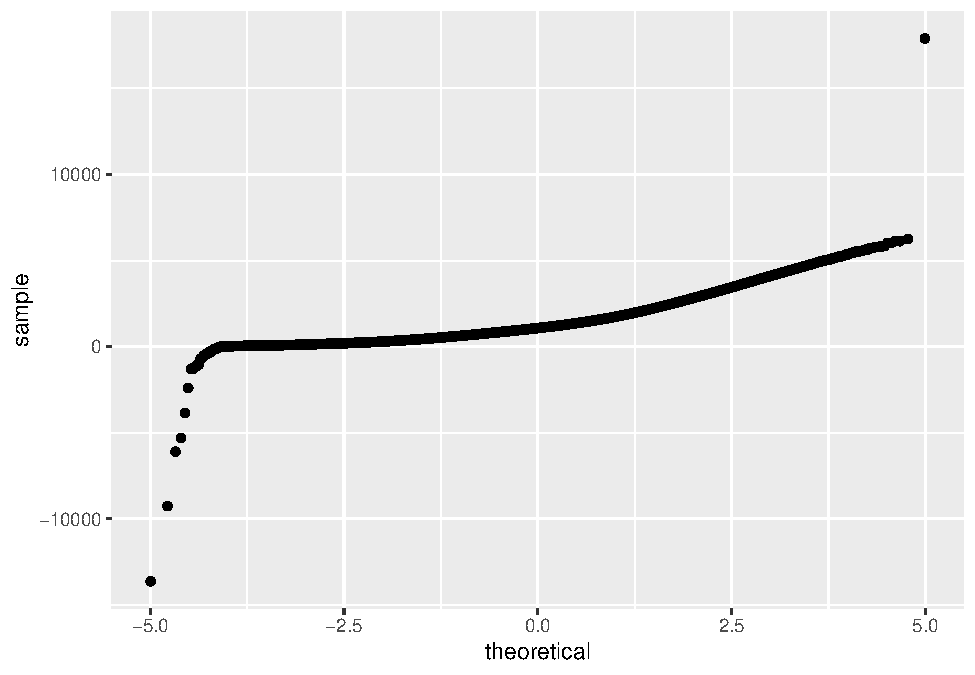
\includegraphics{final_report_files/figure-latex/unnamed-chunk-3-1.pdf}

\begin{Shaded}
\begin{Highlighting}[]
\CommentTok{\# filter out negative and outlying application processing time}
\NormalTok{application\_dates }\OtherTok{\textless{}{-}}\NormalTok{ application\_dates }\SpecialCharTok{\%\textgreater{}\%} 
    \FunctionTok{filter}\NormalTok{(app\_proc\_time}\SpecialCharTok{\textgreater{}}\FunctionTok{ddays}\NormalTok{(}\DecValTok{0}\NormalTok{)) }\SpecialCharTok{\%\textgreater{}\%} 
    \FunctionTok{filter}\NormalTok{(app\_proc\_time}\SpecialCharTok{\textless{}}\FunctionTok{ddays}\NormalTok{(}\DecValTok{10000}\NormalTok{))}

\FunctionTok{head}\NormalTok{(application\_dates) }\CommentTok{\#1,688,672 applications}
\end{Highlighting}
\end{Shaded}

\begin{verbatim}
## # A tibble: 6 x 11
##   application_number filing_date abandon_date patent_issue_date decision_date
##   <chr>              <date>      <date>       <date>            <date>       
## 1 08284457           2000-01-26  NA           2003-02-18        2003-02-18   
## 2 08413193           2000-10-11  NA           2002-08-27        2002-08-27   
## 3 08637752           2001-07-20  NA           2005-08-09        2005-08-09   
## 4 08682726           2000-04-10  2000-12-27   NA                2000-12-27   
## 5 08687412           2000-04-28  NA           2001-07-31        2001-07-31   
## 6 08765941           2000-06-23  2001-08-22   NA                2001-08-22   
## # ... with 6 more variables: examiner_id <dbl>, examiner_art_unit <dbl>,
## #   gender <chr>, race <chr>, tenure_days <dbl>, app_proc_time <drtn>
\end{verbatim}

\begin{Shaded}
\begin{Highlighting}[]
\CommentTok{\# plot again the data distribution of application processing time after cleaning}
\NormalTok{application\_dates }\SpecialCharTok{\%\textgreater{}\%}
  \FunctionTok{ggplot}\NormalTok{(}\FunctionTok{aes}\NormalTok{(}\AttributeTok{sample =}\NormalTok{ app\_proc\_time)) }\SpecialCharTok{+}
  \FunctionTok{geom\_qq}\NormalTok{()}
\end{Highlighting}
\end{Shaded}

\begin{verbatim}
## Don't know how to automatically pick scale for object of type difftime. Defaulting to continuous.
## Don't know how to automatically pick scale for object of type difftime. Defaulting to continuous.
\end{verbatim}

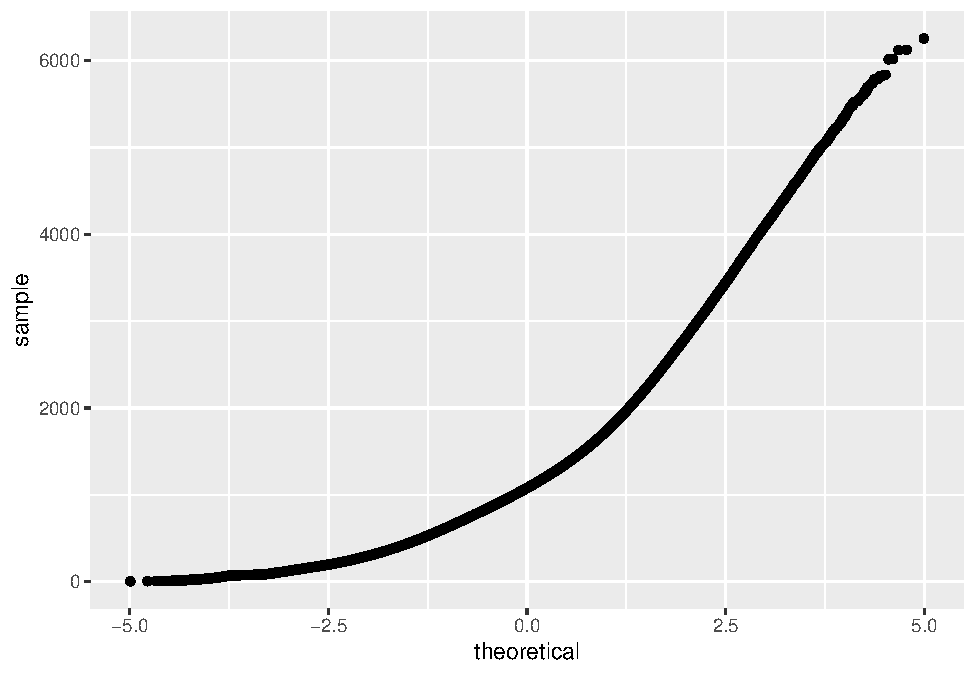
\includegraphics{final_report_files/figure-latex/unnamed-chunk-5-1.pdf}
Outliers are removed successfully.

\hypertarget{get-work-group-from-art-unit}{%
\subsubsection{Get work group from art
unit}\label{get-work-group-from-art-unit}}

\begin{Shaded}
\begin{Highlighting}[]
\CommentTok{\# before we begin, get the workgroup from art unit as rounding down to digit tenth.}
\NormalTok{application\_dates }\OtherTok{\textless{}{-}}\NormalTok{ application\_dates }\SpecialCharTok{\%\textgreater{}\%}
  \FunctionTok{mutate}\NormalTok{(}\AttributeTok{wg =}\NormalTok{ (application\_dates}\SpecialCharTok{$}\NormalTok{examiner\_art\_unit}\SpecialCharTok{\%/\%}\DecValTok{10}\NormalTok{) }\SpecialCharTok{*} \DecValTok{10}\NormalTok{)}

\CommentTok{\# Find out which is the dominating workgroup an examiner handled the applications for.}
\FunctionTok{library}\NormalTok{(plyr)}
\end{Highlighting}
\end{Shaded}

\begin{verbatim}
## ------------------------------------------------------------------------------
\end{verbatim}

\begin{verbatim}
## You have loaded plyr after dplyr - this is likely to cause problems.
## If you need functions from both plyr and dplyr, please load plyr first, then dplyr:
## library(plyr); library(dplyr)
\end{verbatim}

\begin{verbatim}
## ------------------------------------------------------------------------------
\end{verbatim}

\begin{verbatim}
## 
## Attaching package: 'plyr'
\end{verbatim}

\begin{verbatim}
## The following objects are masked from 'package:dplyr':
## 
##     arrange, count, desc, failwith, id, mutate, rename, summarise,
##     summarize
\end{verbatim}

\begin{verbatim}
## The following object is masked from 'package:purrr':
## 
##     compact
\end{verbatim}

\begin{Shaded}
\begin{Highlighting}[]
\FunctionTok{library}\NormalTok{(dplyr)}
\FunctionTok{library}\NormalTok{(lubridate)}
\NormalTok{application\_dates }\OtherTok{\textless{}{-}} \FunctionTok{mutate}\NormalTok{(}
\NormalTok{  application\_dates,}
  \AttributeTok{period =} \FunctionTok{case\_when}\NormalTok{(}
\NormalTok{    filing\_date}\SpecialCharTok{\textless{}}\FunctionTok{ymd}\NormalTok{(}\StringTok{"2007{-}01{-}01"}\NormalTok{) }\SpecialCharTok{\textasciitilde{}} \ConstantTok{NA\_character\_}\NormalTok{,}
\NormalTok{    filing\_date}\SpecialCharTok{\textless{}}\FunctionTok{ymd}\NormalTok{(}\StringTok{"2008{-}01{-}01"}\NormalTok{) }\SpecialCharTok{\textasciitilde{}} \StringTok{"t0"}\NormalTok{,}
\NormalTok{    filing\_date}\SpecialCharTok{\textless{}}\FunctionTok{ymd}\NormalTok{(}\StringTok{"2009{-}01{-}01"}\NormalTok{) }\SpecialCharTok{\textasciitilde{}} \StringTok{"t1"}\NormalTok{,}
\NormalTok{    filing\_date}\SpecialCharTok{\textless{}}\FunctionTok{ymd}\NormalTok{(}\StringTok{"2010{-}01{-}01"}\NormalTok{) }\SpecialCharTok{\textasciitilde{}} \StringTok{"t2"}\NormalTok{,}
\NormalTok{    filing\_date}\SpecialCharTok{\textless{}}\FunctionTok{ymd}\NormalTok{(}\StringTok{"2011{-}01{-}01"}\NormalTok{) }\SpecialCharTok{\textasciitilde{}} \StringTok{"t3"}\NormalTok{,}
\NormalTok{    filing\_date}\SpecialCharTok{\textless{}}\FunctionTok{ymd}\NormalTok{(}\StringTok{"2012{-}01{-}01"}\NormalTok{) }\SpecialCharTok{\textasciitilde{}} \StringTok{"t4"}\NormalTok{,}
\NormalTok{    filing\_date}\SpecialCharTok{\textless{}}\FunctionTok{ymd}\NormalTok{(}\StringTok{"2013{-}01{-}01"}\NormalTok{) }\SpecialCharTok{\textasciitilde{}} \StringTok{"t5"}\NormalTok{,}
\NormalTok{    filing\_date}\SpecialCharTok{\textless{}}\FunctionTok{ymd}\NormalTok{(}\StringTok{"2014{-}01{-}01"}\NormalTok{) }\SpecialCharTok{\textasciitilde{}} \StringTok{"t6"}\NormalTok{,}
\NormalTok{    filing\_date}\SpecialCharTok{\textless{}}\FunctionTok{ymd}\NormalTok{(}\StringTok{"2015{-}01{-}01"}\NormalTok{) }\SpecialCharTok{\textasciitilde{}} \StringTok{"t7"}\NormalTok{,}
\NormalTok{    filing\_date}\SpecialCharTok{\textless{}}\FunctionTok{ymd}\NormalTok{(}\StringTok{"2016{-}01{-}01"}\NormalTok{) }\SpecialCharTok{\textasciitilde{}} \StringTok{"t8"}\NormalTok{,}
    \ConstantTok{TRUE}\SpecialCharTok{\textasciitilde{}} \ConstantTok{NA\_character\_}\NormalTok{)}
\NormalTok{  )}

\CommentTok{\# get number of applications}
\FunctionTok{library}\NormalTok{(plyr)}
\NormalTok{examiner\_wg\_napp }\OtherTok{\textless{}{-}} \FunctionTok{ddply}\NormalTok{(application\_dates, .(examiner\_id, period, wg), nrow)}
\FunctionTok{names}\NormalTok{(examiner\_wg\_napp) }\OtherTok{\textless{}{-}} \FunctionTok{c}\NormalTok{(}\StringTok{"examiner\_id"}\NormalTok{,}\StringTok{"period"}\NormalTok{, }\StringTok{"wg"}\NormalTok{, }\StringTok{"n\_applications"}\NormalTok{)}

\CommentTok{\# assume an examiner belong to the wg he/she most frequently handled applications for, if tie take the greater wg}
\NormalTok{examiner\_wg\_napp }\OtherTok{\textless{}{-}}\NormalTok{ examiner\_wg\_napp[}\FunctionTok{order}\NormalTok{(examiner\_wg\_napp}\SpecialCharTok{$}\NormalTok{examiner\_id, examiner\_wg\_napp}\SpecialCharTok{$}\NormalTok{period, }\SpecialCharTok{{-}}\NormalTok{(examiner\_wg\_napp}\SpecialCharTok{$}\NormalTok{n\_applications), }\SpecialCharTok{{-}}\NormalTok{(examiner\_wg\_napp}\SpecialCharTok{$}\NormalTok{wg)), ] }\DocumentationTok{\#\#\# sort first}
\NormalTok{examiner\_wg }\OtherTok{\textless{}{-}}\NormalTok{ examiner\_wg\_napp [}\SpecialCharTok{!}\FunctionTok{duplicated}\NormalTok{(examiner\_wg\_napp[}\FunctionTok{c}\NormalTok{(}\DecValTok{1}\NormalTok{,}\DecValTok{2}\NormalTok{)]),]}
\NormalTok{examiner\_wg }\OtherTok{\textless{}{-}} \FunctionTok{select}\NormalTok{(examiner\_wg, }\FunctionTok{c}\NormalTok{(}\StringTok{"examiner\_id"}\NormalTok{,}\StringTok{"wg"}\NormalTok{,}\StringTok{"period"}\NormalTok{))}
\NormalTok{examiner\_wg }\OtherTok{\textless{}{-}} \FunctionTok{drop\_na}\NormalTok{(examiner\_wg)}

\FunctionTok{rm}\NormalTok{(examiner\_wg\_napp)}
\end{Highlighting}
\end{Shaded}

\hypertarget{get-seniority-at-each-period}{%
\subsubsection{Get seniority at each
period}\label{get-seniority-at-each-period}}

Let's assume a time period of \(t_0 = 2007\) (the year we first get
senior examiners, according to our definition), \(t_1 = 2008\),
\(t_2 = 2009\), \(t_3 = 2010\), \(t_4 = 2011\), \(t_5 = 2012\),
\(t_6 = 2013\), \(t_7 = 2014\), \(t_8 = 2015\)

\begin{Shaded}
\begin{Highlighting}[]
\CommentTok{\# Get tenure \& state at each period}
\NormalTok{examiner\_dates }\OtherTok{\textless{}{-}}\NormalTok{ examiner\_dates }\SpecialCharTok{\%\textgreater{}\%} 
  \FunctionTok{mutate}\NormalTok{(}
    \AttributeTok{tenure\_t0 =} \FunctionTok{ifelse}\NormalTok{(}\FunctionTok{as.duration}\NormalTok{(earliest\_date }\SpecialCharTok{\%{-}{-}\%} \FunctionTok{ymd}\NormalTok{(}\StringTok{"2007{-}01{-}01"}\NormalTok{)) }\SpecialCharTok{/} \FunctionTok{dyears}\NormalTok{(}\DecValTok{1}\NormalTok{)}\SpecialCharTok{\textless{}}\DecValTok{0}\NormalTok{,}\DecValTok{0}\NormalTok{,}\FunctionTok{as.duration}\NormalTok{(earliest\_date }\SpecialCharTok{\%{-}{-}\%} \FunctionTok{ymd}\NormalTok{(}\StringTok{"2007{-}01{-}01"}\NormalTok{))}\SpecialCharTok{/}\FunctionTok{dyears}\NormalTok{(}\DecValTok{1}\NormalTok{)),}
    \AttributeTok{tenure\_t1 =} \FunctionTok{ifelse}\NormalTok{(}\FunctionTok{as.duration}\NormalTok{(earliest\_date }\SpecialCharTok{\%{-}{-}\%} \FunctionTok{ymd}\NormalTok{(}\StringTok{"2008{-}01{-}01"}\NormalTok{)) }\SpecialCharTok{/} \FunctionTok{dyears}\NormalTok{(}\DecValTok{1}\NormalTok{)}\SpecialCharTok{\textless{}}\DecValTok{0}\NormalTok{,}\DecValTok{0}\NormalTok{,}\FunctionTok{as.duration}\NormalTok{(earliest\_date }\SpecialCharTok{\%{-}{-}\%} \FunctionTok{ymd}\NormalTok{(}\StringTok{"2008{-}01{-}01"}\NormalTok{))}\SpecialCharTok{/}\FunctionTok{dyears}\NormalTok{(}\DecValTok{1}\NormalTok{)),}
    \AttributeTok{tenure\_t2 =} \FunctionTok{ifelse}\NormalTok{(}\FunctionTok{as.duration}\NormalTok{(earliest\_date }\SpecialCharTok{\%{-}{-}\%} \FunctionTok{ymd}\NormalTok{(}\StringTok{"2009{-}01{-}01"}\NormalTok{)) }\SpecialCharTok{/} \FunctionTok{dyears}\NormalTok{(}\DecValTok{1}\NormalTok{)}\SpecialCharTok{\textless{}}\DecValTok{0}\NormalTok{,}\DecValTok{0}\NormalTok{,}\FunctionTok{as.duration}\NormalTok{(earliest\_date }\SpecialCharTok{\%{-}{-}\%} \FunctionTok{ymd}\NormalTok{(}\StringTok{"2009{-}01{-}01"}\NormalTok{))}\SpecialCharTok{/}\FunctionTok{dyears}\NormalTok{(}\DecValTok{1}\NormalTok{)),}
    \AttributeTok{tenure\_t3 =} \FunctionTok{ifelse}\NormalTok{(}\FunctionTok{as.duration}\NormalTok{(earliest\_date }\SpecialCharTok{\%{-}{-}\%} \FunctionTok{ymd}\NormalTok{(}\StringTok{"2010{-}01{-}01"}\NormalTok{)) }\SpecialCharTok{/} \FunctionTok{dyears}\NormalTok{(}\DecValTok{1}\NormalTok{)}\SpecialCharTok{\textless{}}\DecValTok{0}\NormalTok{,}\DecValTok{0}\NormalTok{,}\FunctionTok{as.duration}\NormalTok{(earliest\_date }\SpecialCharTok{\%{-}{-}\%} \FunctionTok{ymd}\NormalTok{(}\StringTok{"2010{-}01{-}01"}\NormalTok{))}\SpecialCharTok{/}\FunctionTok{dyears}\NormalTok{(}\DecValTok{1}\NormalTok{)),}
    \AttributeTok{tenure\_t4 =} \FunctionTok{ifelse}\NormalTok{(}\FunctionTok{as.duration}\NormalTok{(earliest\_date }\SpecialCharTok{\%{-}{-}\%} \FunctionTok{ymd}\NormalTok{(}\StringTok{"2011{-}01{-}01"}\NormalTok{)) }\SpecialCharTok{/} \FunctionTok{dyears}\NormalTok{(}\DecValTok{1}\NormalTok{)}\SpecialCharTok{\textless{}}\DecValTok{0}\NormalTok{,}\DecValTok{0}\NormalTok{,}\FunctionTok{as.duration}\NormalTok{(earliest\_date }\SpecialCharTok{\%{-}{-}\%} \FunctionTok{ymd}\NormalTok{(}\StringTok{"2011{-}01{-}01"}\NormalTok{))}\SpecialCharTok{/}\FunctionTok{dyears}\NormalTok{(}\DecValTok{1}\NormalTok{)),}
    \AttributeTok{tenure\_t5 =} \FunctionTok{ifelse}\NormalTok{(}\FunctionTok{as.duration}\NormalTok{(earliest\_date }\SpecialCharTok{\%{-}{-}\%} \FunctionTok{ymd}\NormalTok{(}\StringTok{"2012{-}01{-}01"}\NormalTok{)) }\SpecialCharTok{/} \FunctionTok{dyears}\NormalTok{(}\DecValTok{1}\NormalTok{)}\SpecialCharTok{\textless{}}\DecValTok{0}\NormalTok{,}\DecValTok{0}\NormalTok{,}\FunctionTok{as.duration}\NormalTok{(earliest\_date }\SpecialCharTok{\%{-}{-}\%} \FunctionTok{ymd}\NormalTok{(}\StringTok{"2012{-}01{-}01"}\NormalTok{))}\SpecialCharTok{/}\FunctionTok{dyears}\NormalTok{(}\DecValTok{1}\NormalTok{)),}
    \AttributeTok{tenure\_t6 =} \FunctionTok{ifelse}\NormalTok{(}\FunctionTok{as.duration}\NormalTok{(earliest\_date }\SpecialCharTok{\%{-}{-}\%} \FunctionTok{ymd}\NormalTok{(}\StringTok{"2013{-}01{-}01"}\NormalTok{)) }\SpecialCharTok{/} \FunctionTok{dyears}\NormalTok{(}\DecValTok{1}\NormalTok{)}\SpecialCharTok{\textless{}}\DecValTok{0}\NormalTok{,}\DecValTok{0}\NormalTok{,}\FunctionTok{as.duration}\NormalTok{(earliest\_date }\SpecialCharTok{\%{-}{-}\%} \FunctionTok{ymd}\NormalTok{(}\StringTok{"2013{-}01{-}01"}\NormalTok{))}\SpecialCharTok{/}\FunctionTok{dyears}\NormalTok{(}\DecValTok{1}\NormalTok{)),}
    \AttributeTok{tenure\_t7 =} \FunctionTok{ifelse}\NormalTok{(}\FunctionTok{as.duration}\NormalTok{(earliest\_date }\SpecialCharTok{\%{-}{-}\%} \FunctionTok{ymd}\NormalTok{(}\StringTok{"2014{-}01{-}01"}\NormalTok{)) }\SpecialCharTok{/} \FunctionTok{dyears}\NormalTok{(}\DecValTok{1}\NormalTok{)}\SpecialCharTok{\textless{}}\DecValTok{0}\NormalTok{,}\DecValTok{0}\NormalTok{,}\FunctionTok{as.duration}\NormalTok{(earliest\_date }\SpecialCharTok{\%{-}{-}\%} \FunctionTok{ymd}\NormalTok{(}\StringTok{"2014{-}01{-}01"}\NormalTok{))}\SpecialCharTok{/}\FunctionTok{dyears}\NormalTok{(}\DecValTok{1}\NormalTok{)),}
    \AttributeTok{tenure\_t8 =} \FunctionTok{ifelse}\NormalTok{(}\FunctionTok{as.duration}\NormalTok{(earliest\_date }\SpecialCharTok{\%{-}{-}\%} \FunctionTok{ymd}\NormalTok{(}\StringTok{"2015{-}01{-}01"}\NormalTok{)) }\SpecialCharTok{/} \FunctionTok{dyears}\NormalTok{(}\DecValTok{1}\NormalTok{)}\SpecialCharTok{\textless{}}\DecValTok{0}\NormalTok{,}\DecValTok{0}\NormalTok{,}\FunctionTok{as.duration}\NormalTok{(earliest\_date }\SpecialCharTok{\%{-}{-}\%} \FunctionTok{ymd}\NormalTok{(}\StringTok{"2015{-}01{-}01"}\NormalTok{))}\SpecialCharTok{/}\FunctionTok{dyears}\NormalTok{(}\DecValTok{1}\NormalTok{)),}

    \AttributeTok{t0\_state =} \FunctionTok{case\_when}\NormalTok{(}
\NormalTok{      tenure\_t0}\SpecialCharTok{\textless{}}\DecValTok{6} \SpecialCharTok{\&}\NormalTok{ tenure\_t0}\SpecialCharTok{\textgreater{}}\DecValTok{0} \SpecialCharTok{\textasciitilde{}} \StringTok{"Junior"}\NormalTok{  , }\CommentTok{\# Jr; not those yet to be hired!}
\NormalTok{      tenure\_t0}\SpecialCharTok{\textgreater{}=}\DecValTok{6}              \SpecialCharTok{\textasciitilde{}} \StringTok{"Senior"}\NormalTok{  , }\CommentTok{\# Sr}
      \ConstantTok{TRUE}                      \SpecialCharTok{\textasciitilde{}} \ConstantTok{NA\_character\_} \CommentTok{\# not yet hired}
\NormalTok{    ),}
    \AttributeTok{t1\_state =} \FunctionTok{case\_when}\NormalTok{(}
\NormalTok{      latest\_date}\SpecialCharTok{\textless{}}\FunctionTok{ymd}\NormalTok{(}\StringTok{"2008{-}12{-}31"}\NormalTok{)        }\SpecialCharTok{\textasciitilde{}} \StringTok{"Exit"}\NormalTok{,}
\NormalTok{      earliest\_date}\SpecialCharTok{\textgreater{}}\FunctionTok{ymd}\NormalTok{(}\StringTok{"2007{-}01{-}01"}\NormalTok{) }
        \SpecialCharTok{\&}\NormalTok{ earliest\_date}\SpecialCharTok{\textless{}}\FunctionTok{ymd}\NormalTok{(}\StringTok{"2008{-}01{-}01"}\NormalTok{) }\SpecialCharTok{\textasciitilde{}} \StringTok{"New hire"}\NormalTok{,}
\NormalTok{      tenure\_t1}\SpecialCharTok{\textless{}}\DecValTok{6} \SpecialCharTok{\&}\NormalTok{ tenure\_t1}\SpecialCharTok{\textgreater{}}\DecValTok{0}          \SpecialCharTok{\textasciitilde{}} \StringTok{"Junior"}\NormalTok{  , }\CommentTok{\# Jr; not those yet to be hired!}
\NormalTok{      tenure\_t1}\SpecialCharTok{\textgreater{}=}\DecValTok{6}                       \SpecialCharTok{\textasciitilde{}} \StringTok{"Senior"}\NormalTok{  , }\CommentTok{\# Sr}
      \ConstantTok{TRUE}                               \SpecialCharTok{\textasciitilde{}} \ConstantTok{NA\_character\_} \CommentTok{\# not yet hired}
\NormalTok{      ),}
    \AttributeTok{t2\_state =} \FunctionTok{case\_when}\NormalTok{(}
\NormalTok{      t1\_state}\SpecialCharTok{==}\StringTok{"Exit"}                   \SpecialCharTok{\textasciitilde{}} \ConstantTok{NA\_character\_}\NormalTok{,}
\NormalTok{      latest\_date}\SpecialCharTok{\textless{}}\FunctionTok{ymd}\NormalTok{(}\StringTok{"2009{-}12{-}31"}\NormalTok{)        }\SpecialCharTok{\textasciitilde{}} \StringTok{"Exit"}\NormalTok{,}
\NormalTok{      earliest\_date}\SpecialCharTok{\textgreater{}}\FunctionTok{ymd}\NormalTok{(}\StringTok{"2008{-}01{-}01"}\NormalTok{) }
        \SpecialCharTok{\&}\NormalTok{ earliest\_date}\SpecialCharTok{\textless{}}\FunctionTok{ymd}\NormalTok{(}\StringTok{"2009{-}01{-}01"}\NormalTok{) }\SpecialCharTok{\textasciitilde{}} \StringTok{"New hire"}\NormalTok{,}
\NormalTok{      tenure\_t2}\SpecialCharTok{\textless{}}\DecValTok{6} \SpecialCharTok{\&}\NormalTok{ tenure\_t2}\SpecialCharTok{\textgreater{}}\DecValTok{0}          \SpecialCharTok{\textasciitilde{}} \StringTok{"Junior"}\NormalTok{  , }\CommentTok{\# Jr; not those yet to be hired!}
\NormalTok{      tenure\_t2}\SpecialCharTok{\textgreater{}=}\DecValTok{6}                       \SpecialCharTok{\textasciitilde{}} \StringTok{"Senior"}\NormalTok{  , }\CommentTok{\# Sr}
      \ConstantTok{TRUE}                               \SpecialCharTok{\textasciitilde{}} \ConstantTok{NA\_character\_} \CommentTok{\# not yet hired or already exit in previous period}
\NormalTok{      ),}
    \AttributeTok{t3\_state =} \FunctionTok{case\_when}\NormalTok{(}
\NormalTok{      t1\_state}\SpecialCharTok{==}\StringTok{"Exit"}\SpecialCharTok{|}\NormalTok{t2\_state}\SpecialCharTok{==}\StringTok{"Exit"}                   \SpecialCharTok{\textasciitilde{}} \ConstantTok{NA\_character\_}\NormalTok{,}
\NormalTok{      latest\_date}\SpecialCharTok{\textless{}}\FunctionTok{ymd}\NormalTok{(}\StringTok{"2010{-}12{-}31"}\NormalTok{)        }\SpecialCharTok{\textasciitilde{}} \StringTok{"Exit"}\NormalTok{,}
\NormalTok{      earliest\_date}\SpecialCharTok{\textgreater{}}\FunctionTok{ymd}\NormalTok{(}\StringTok{"2009{-}01{-}01"}\NormalTok{) }
        \SpecialCharTok{\&}\NormalTok{ earliest\_date}\SpecialCharTok{\textless{}}\FunctionTok{ymd}\NormalTok{(}\StringTok{"2010{-}01{-}01"}\NormalTok{) }\SpecialCharTok{\textasciitilde{}} \StringTok{"New hire"}\NormalTok{,}
\NormalTok{      tenure\_t3}\SpecialCharTok{\textless{}}\DecValTok{6} \SpecialCharTok{\&}\NormalTok{ tenure\_t3}\SpecialCharTok{\textgreater{}}\DecValTok{0}          \SpecialCharTok{\textasciitilde{}} \StringTok{"Junior"}\NormalTok{  , }\CommentTok{\# Jr; not those yet to be hired!}
\NormalTok{      tenure\_t3}\SpecialCharTok{\textgreater{}=}\DecValTok{6}                       \SpecialCharTok{\textasciitilde{}} \StringTok{"Senior"}\NormalTok{  , }\CommentTok{\# Sr}
      \ConstantTok{TRUE}                               \SpecialCharTok{\textasciitilde{}} \ConstantTok{NA\_character\_} \CommentTok{\# not yet hired or already exit in previous period}
\NormalTok{      ),}
    \AttributeTok{t4\_state =} \FunctionTok{case\_when}\NormalTok{(}
\NormalTok{      t1\_state}\SpecialCharTok{==}\StringTok{"Exit"}\SpecialCharTok{|}\NormalTok{t2\_state}\SpecialCharTok{==}\StringTok{"Exit"}\SpecialCharTok{|}\NormalTok{t3\_state}\SpecialCharTok{==}\StringTok{"Exit"}                   \SpecialCharTok{\textasciitilde{}} \ConstantTok{NA\_character\_}\NormalTok{,}
\NormalTok{      latest\_date}\SpecialCharTok{\textless{}}\FunctionTok{ymd}\NormalTok{(}\StringTok{"2011{-}12{-}31"}\NormalTok{)        }\SpecialCharTok{\textasciitilde{}} \StringTok{"Exit"}\NormalTok{,}
\NormalTok{      earliest\_date}\SpecialCharTok{\textgreater{}}\FunctionTok{ymd}\NormalTok{(}\StringTok{"2010{-}01{-}01"}\NormalTok{) }
        \SpecialCharTok{\&}\NormalTok{ earliest\_date}\SpecialCharTok{\textless{}}\FunctionTok{ymd}\NormalTok{(}\StringTok{"2011{-}01{-}01"}\NormalTok{) }\SpecialCharTok{\textasciitilde{}} \StringTok{"New hire"}\NormalTok{,}
\NormalTok{      tenure\_t4}\SpecialCharTok{\textless{}}\DecValTok{6} \SpecialCharTok{\&}\NormalTok{ tenure\_t4}\SpecialCharTok{\textgreater{}}\DecValTok{0}          \SpecialCharTok{\textasciitilde{}} \StringTok{"Junior"}\NormalTok{  , }\CommentTok{\# Jr; not those yet to be hired!}
\NormalTok{      tenure\_t4}\SpecialCharTok{\textgreater{}=}\DecValTok{6}                       \SpecialCharTok{\textasciitilde{}} \StringTok{"Senior"}\NormalTok{  , }\CommentTok{\# Sr}
      \ConstantTok{TRUE}                               \SpecialCharTok{\textasciitilde{}} \ConstantTok{NA\_character\_} \CommentTok{\# not yet hired or already exit in previous period}
\NormalTok{      ),}
    \AttributeTok{t5\_state =} \FunctionTok{case\_when}\NormalTok{(}
\NormalTok{      t1\_state}\SpecialCharTok{==}\StringTok{"Exit"}\SpecialCharTok{|}\NormalTok{t2\_state}\SpecialCharTok{==}\StringTok{"Exit"}\SpecialCharTok{|}\NormalTok{t3\_state}\SpecialCharTok{==}\StringTok{"Exit"}\SpecialCharTok{|}\NormalTok{t4\_state}\SpecialCharTok{==}\StringTok{"Exit"}                   \SpecialCharTok{\textasciitilde{}} \ConstantTok{NA\_character\_}\NormalTok{,}
\NormalTok{      latest\_date}\SpecialCharTok{\textless{}}\FunctionTok{ymd}\NormalTok{(}\StringTok{"2012{-}12{-}31"}\NormalTok{)        }\SpecialCharTok{\textasciitilde{}} \StringTok{"Exit"}\NormalTok{,}
\NormalTok{      earliest\_date}\SpecialCharTok{\textgreater{}}\FunctionTok{ymd}\NormalTok{(}\StringTok{"2011{-}01{-}01"}\NormalTok{) }
        \SpecialCharTok{\&}\NormalTok{ earliest\_date}\SpecialCharTok{\textless{}}\FunctionTok{ymd}\NormalTok{(}\StringTok{"2012{-}01{-}01"}\NormalTok{) }\SpecialCharTok{\textasciitilde{}} \StringTok{"New hire"}\NormalTok{,}
\NormalTok{      tenure\_t5}\SpecialCharTok{\textless{}}\DecValTok{6} \SpecialCharTok{\&}\NormalTok{ tenure\_t5}\SpecialCharTok{\textgreater{}}\DecValTok{0}          \SpecialCharTok{\textasciitilde{}} \StringTok{"Junior"}\NormalTok{  , }\CommentTok{\# Jr; not those yet to be hired!}
\NormalTok{      tenure\_t5}\SpecialCharTok{\textgreater{}=}\DecValTok{6}                       \SpecialCharTok{\textasciitilde{}} \StringTok{"Senior"}\NormalTok{  , }\CommentTok{\# Sr}
      \ConstantTok{TRUE}                               \SpecialCharTok{\textasciitilde{}} \ConstantTok{NA\_character\_} \CommentTok{\# not yet hired or already exit in previous period}
\NormalTok{      ),}
    \AttributeTok{t6\_state =} \FunctionTok{case\_when}\NormalTok{(}
\NormalTok{      t1\_state}\SpecialCharTok{==}\StringTok{"Exit"}\SpecialCharTok{|}\NormalTok{t2\_state}\SpecialCharTok{==}\StringTok{"Exit"}\SpecialCharTok{|}\NormalTok{t3\_state}\SpecialCharTok{==}\StringTok{"Exit"}\SpecialCharTok{|}\NormalTok{t4\_state}\SpecialCharTok{==}\StringTok{"Exit"}\SpecialCharTok{|}\NormalTok{t5\_state}\SpecialCharTok{==}\StringTok{"Exit"}                   \SpecialCharTok{\textasciitilde{}} \ConstantTok{NA\_character\_}\NormalTok{,}
\NormalTok{      latest\_date}\SpecialCharTok{\textless{}}\FunctionTok{ymd}\NormalTok{(}\StringTok{"2013{-}12{-}31"}\NormalTok{)        }\SpecialCharTok{\textasciitilde{}} \StringTok{"Exit"}\NormalTok{,}
\NormalTok{      earliest\_date}\SpecialCharTok{\textgreater{}}\FunctionTok{ymd}\NormalTok{(}\StringTok{"2012{-}01{-}01"}\NormalTok{) }
        \SpecialCharTok{\&}\NormalTok{ earliest\_date}\SpecialCharTok{\textless{}}\FunctionTok{ymd}\NormalTok{(}\StringTok{"2013{-}01{-}01"}\NormalTok{) }\SpecialCharTok{\textasciitilde{}} \StringTok{"New hire"}\NormalTok{,}
\NormalTok{      tenure\_t6}\SpecialCharTok{\textless{}}\DecValTok{6} \SpecialCharTok{\&}\NormalTok{ tenure\_t6}\SpecialCharTok{\textgreater{}}\DecValTok{0}          \SpecialCharTok{\textasciitilde{}} \StringTok{"Junior"}\NormalTok{  , }\CommentTok{\# Jr; not those yet to be hired!}
\NormalTok{      tenure\_t6}\SpecialCharTok{\textgreater{}=}\DecValTok{6}                       \SpecialCharTok{\textasciitilde{}} \StringTok{"Senior"}\NormalTok{  , }\CommentTok{\# Sr}
      \ConstantTok{TRUE}                               \SpecialCharTok{\textasciitilde{}} \ConstantTok{NA\_character\_} \CommentTok{\# not yet hired or already exit in previous period}
\NormalTok{      ),}
    \AttributeTok{t7\_state =} \FunctionTok{case\_when}\NormalTok{(}
\NormalTok{      t1\_state}\SpecialCharTok{==}\StringTok{"Exit"}\SpecialCharTok{|}\NormalTok{t2\_state}\SpecialCharTok{==}\StringTok{"Exit"}\SpecialCharTok{|}\NormalTok{t3\_state}\SpecialCharTok{==}\StringTok{"Exit"}\SpecialCharTok{|}\NormalTok{t4\_state}\SpecialCharTok{==}\StringTok{"Exit"}\SpecialCharTok{|}\NormalTok{t5\_state}\SpecialCharTok{==}\StringTok{"Exit"}\SpecialCharTok{|}\NormalTok{t6\_state}\SpecialCharTok{==}\StringTok{"Exit"}                   \SpecialCharTok{\textasciitilde{}} \ConstantTok{NA\_character\_}\NormalTok{,}
\NormalTok{      latest\_date}\SpecialCharTok{\textless{}}\FunctionTok{ymd}\NormalTok{(}\StringTok{"2014{-}12{-}31"}\NormalTok{)        }\SpecialCharTok{\textasciitilde{}} \StringTok{"Exit"}\NormalTok{,}
\NormalTok{      earliest\_date}\SpecialCharTok{\textgreater{}}\FunctionTok{ymd}\NormalTok{(}\StringTok{"2013{-}01{-}01"}\NormalTok{) }
        \SpecialCharTok{\&}\NormalTok{ earliest\_date}\SpecialCharTok{\textless{}}\FunctionTok{ymd}\NormalTok{(}\StringTok{"2014{-}01{-}01"}\NormalTok{) }\SpecialCharTok{\textasciitilde{}} \StringTok{"New hire"}\NormalTok{,}
\NormalTok{      tenure\_t7}\SpecialCharTok{\textless{}}\DecValTok{6} \SpecialCharTok{\&}\NormalTok{ tenure\_t7}\SpecialCharTok{\textgreater{}}\DecValTok{0}          \SpecialCharTok{\textasciitilde{}} \StringTok{"Junior"}\NormalTok{  , }\CommentTok{\# Jr; not those yet to be hired!}
\NormalTok{      tenure\_t7}\SpecialCharTok{\textgreater{}=}\DecValTok{6}                       \SpecialCharTok{\textasciitilde{}} \StringTok{"Senior"}\NormalTok{  , }\CommentTok{\# Sr}
      \ConstantTok{TRUE}                               \SpecialCharTok{\textasciitilde{}} \ConstantTok{NA\_character\_} \CommentTok{\# not yet hired or already exit in previous period}
\NormalTok{      ),}
    \AttributeTok{t8\_state =} \FunctionTok{case\_when}\NormalTok{(}
\NormalTok{      t1\_state}\SpecialCharTok{==}\StringTok{"Exit"}\SpecialCharTok{|}\NormalTok{t2\_state}\SpecialCharTok{==}\StringTok{"Exit"}\SpecialCharTok{|}\NormalTok{t3\_state}\SpecialCharTok{==}\StringTok{"Exit"}\SpecialCharTok{|}\NormalTok{t4\_state}\SpecialCharTok{==}\StringTok{"Exit"}\SpecialCharTok{|}\NormalTok{t5\_state}\SpecialCharTok{==}\StringTok{"Exit"}\SpecialCharTok{|}\NormalTok{t6\_state}\SpecialCharTok{==}\StringTok{"Exit"}\SpecialCharTok{|}\NormalTok{t7\_state}\SpecialCharTok{==}\StringTok{"Exit"}                   \SpecialCharTok{\textasciitilde{}} \ConstantTok{NA\_character\_}\NormalTok{,}
\NormalTok{      latest\_date}\SpecialCharTok{\textless{}}\FunctionTok{ymd}\NormalTok{(}\StringTok{"2015{-}12{-}31"}\NormalTok{)        }\SpecialCharTok{\textasciitilde{}} \StringTok{"Exit"}\NormalTok{,}
\NormalTok{      earliest\_date}\SpecialCharTok{\textgreater{}}\FunctionTok{ymd}\NormalTok{(}\StringTok{"2014{-}01{-}01"}\NormalTok{) }
        \SpecialCharTok{\&}\NormalTok{ earliest\_date}\SpecialCharTok{\textless{}}\FunctionTok{ymd}\NormalTok{(}\StringTok{"2015{-}01{-}01"}\NormalTok{) }\SpecialCharTok{\textasciitilde{}} \StringTok{"New hire"}\NormalTok{,}
\NormalTok{      tenure\_t8}\SpecialCharTok{\textless{}}\DecValTok{6} \SpecialCharTok{\&}\NormalTok{ tenure\_t8}\SpecialCharTok{\textgreater{}}\DecValTok{0}          \SpecialCharTok{\textasciitilde{}} \StringTok{"Junior"}\NormalTok{  , }\CommentTok{\# Jr; not those yet to be hired!}
\NormalTok{      tenure\_t8}\SpecialCharTok{\textgreater{}=}\DecValTok{6}                       \SpecialCharTok{\textasciitilde{}} \StringTok{"Senior"}\NormalTok{  , }\CommentTok{\# Sr}
      \ConstantTok{TRUE}                               \SpecialCharTok{\textasciitilde{}} \ConstantTok{NA\_character\_} \CommentTok{\# not yet hired or already exit in previous period}
\NormalTok{      )}
\NormalTok{    )}

\NormalTok{examiner\_dates }\OtherTok{\textless{}{-}}\NormalTok{ examiner\_dates }\SpecialCharTok{\%\textgreater{}\%} 
  \FunctionTok{select}\NormalTok{(examiner\_id, t0\_state, t1\_state, t2\_state, t3\_state, t4\_state, t5\_state, t6\_state, t7\_state, t8\_state)}

\DocumentationTok{\#\# plot seniority}
\FunctionTok{library}\NormalTok{(ggplot2)}
\FunctionTok{library}\NormalTok{(scales)  }
\end{Highlighting}
\end{Shaded}

\begin{verbatim}
## 
## Attaching package: 'scales'
\end{verbatim}

\begin{verbatim}
## The following object is masked from 'package:purrr':
## 
##     discard
\end{verbatim}

\begin{verbatim}
## The following object is masked from 'package:readr':
## 
##     col_factor
\end{verbatim}

\begin{Shaded}
\begin{Highlighting}[]
\FunctionTok{library}\NormalTok{(gridExtra)}
\end{Highlighting}
\end{Shaded}

\begin{verbatim}
## 
## Attaching package: 'gridExtra'
\end{verbatim}

\begin{verbatim}
## The following object is masked from 'package:dplyr':
## 
##     combine
\end{verbatim}

\begin{Shaded}
\begin{Highlighting}[]
\NormalTok{plot1 }\OtherTok{\textless{}{-}} \FunctionTok{ggplot}\NormalTok{(examiner\_dates, }\FunctionTok{aes}\NormalTok{(}\FunctionTok{factor}\NormalTok{(t1\_state, }\AttributeTok{levels =} \FunctionTok{c}\NormalTok{(}\StringTok{"New hire"}\NormalTok{, }\StringTok{"Junior"}\NormalTok{, }\StringTok{"Senior"}\NormalTok{, }\StringTok{"Exit"}\NormalTok{, }\ConstantTok{NA}\NormalTok{)))) }\SpecialCharTok{+} 
          \FunctionTok{geom\_bar}\NormalTok{(}\FunctionTok{aes}\NormalTok{(}\AttributeTok{y =}\NormalTok{ (..count..)}\SpecialCharTok{/}\FunctionTok{sum}\NormalTok{(..count..))) }\SpecialCharTok{+} 
          \FunctionTok{scale\_y\_continuous}\NormalTok{(}\AttributeTok{labels=}\NormalTok{scales}\SpecialCharTok{::}\NormalTok{percent) }\SpecialCharTok{+}
          \FunctionTok{ylab}\NormalTok{(}\StringTok{"Relative Frequencies"}\NormalTok{) }\SpecialCharTok{+}
          \FunctionTok{ggtitle}\NormalTok{(}\StringTok{"Seniority distribution for USPTO at t1"}\NormalTok{)}
\NormalTok{plot1}
\end{Highlighting}
\end{Shaded}

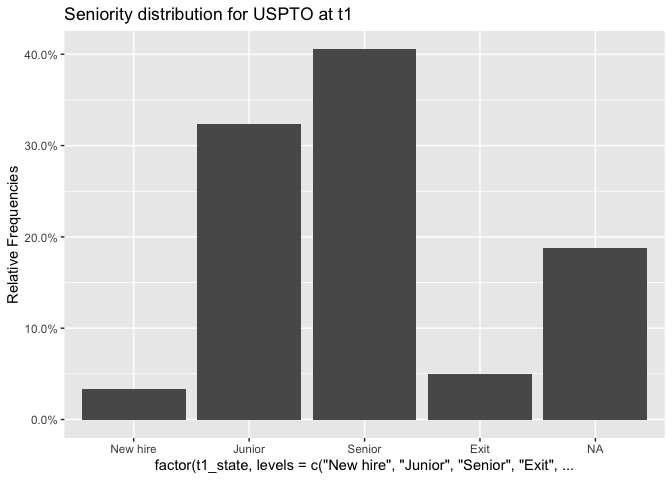
\includegraphics{final_report_files/figure-latex/unnamed-chunk-7-1.pdf}

Joining back to the applications dates data.

\begin{Shaded}
\begin{Highlighting}[]
\NormalTok{application\_dates }\OtherTok{\textless{}{-}}\NormalTok{ application\_dates }\SpecialCharTok{\%\textgreater{}\%} 
  \FunctionTok{left\_join}\NormalTok{(examiner\_dates, }\AttributeTok{by =} \StringTok{"examiner\_id"}\NormalTok{)}
\FunctionTok{rm}\NormalTok{(examiner\_dates)}
\FunctionTok{rm}\NormalTok{(plot1)}
\CommentTok{\#gc()}
\end{Highlighting}
\end{Shaded}

\hypertarget{generate-examiner-panel-dataset}{%
\subsubsection{Generate examiner panel
dataset}\label{generate-examiner-panel-dataset}}

\begin{Shaded}
\begin{Highlighting}[]
\CommentTok{\# compute average application processing time}

\NormalTok{cols }\OtherTok{\textless{}{-}} \FunctionTok{c}\NormalTok{(}\StringTok{"examiner\_id"}\NormalTok{,}\StringTok{"period"}\NormalTok{, }\StringTok{"wg"}\NormalTok{, }\StringTok{"examiner\_art\_unit"}\NormalTok{,}\StringTok{"gender"}\NormalTok{, }\StringTok{"race"}\NormalTok{, }\StringTok{"tenure\_days"}\NormalTok{,}
          \StringTok{"t0\_state"}\NormalTok{,}\StringTok{"t1\_state"}\NormalTok{,}\StringTok{"t2\_state"}\NormalTok{,}\StringTok{"t3\_state"}\NormalTok{,}\StringTok{"t4\_state"}\NormalTok{,}\StringTok{"t5\_state"}\NormalTok{,}\StringTok{"t6\_state"}\NormalTok{,}\StringTok{"t7\_state"}\NormalTok{,}\StringTok{"t8\_state"}\NormalTok{)}

\NormalTok{examiners }\OtherTok{\textless{}{-}}\NormalTok{ application\_dates }\SpecialCharTok{\%\textgreater{}\%}
    \FunctionTok{group\_by}\NormalTok{(}\FunctionTok{across}\NormalTok{(}\FunctionTok{all\_of}\NormalTok{(cols))) }\SpecialCharTok{\%\textgreater{}\%}
\NormalTok{    dplyr}\SpecialCharTok{::}\FunctionTok{summarize}\NormalTok{(}\AttributeTok{mean\_app\_proc\_time =} \FunctionTok{mean}\NormalTok{(app\_proc\_time, }\AttributeTok{na.rm=}\ConstantTok{TRUE}\NormalTok{), }\AttributeTok{n\_app =} \FunctionTok{n}\NormalTok{()) }\SpecialCharTok{\%\textgreater{}\%}
    \FunctionTok{drop\_na}\NormalTok{()}
\end{Highlighting}
\end{Shaded}

\begin{verbatim}
## `summarise()` has grouped output by 'examiner_id', 'period', 'wg', 'examiner_art_unit', 'gender', 'race', 'tenure_days', 't0_state', 't1_state', 't2_state', 't3_state', 't4_state', 't5_state', 't6_state', 't7_state'. You can override using the `.groups` argument.
\end{verbatim}

\begin{Shaded}
\begin{Highlighting}[]
\FunctionTok{head}\NormalTok{(}\FunctionTok{data.frame}\NormalTok{(examiners))}
\end{Highlighting}
\end{Shaded}

\begin{verbatim}
##   examiner_id period   wg examiner_art_unit gender  race tenure_days t0_state
## 1       59012     t0 1710              1716   male white        4013   Junior
## 2       59012     t0 1710              1717   male white        4013   Junior
## 3       59012     t1 1710              1716   male white        4013   Junior
## 4       59012     t1 1710              1717   male white        4013   Junior
## 5       59012     t3 1710              1716   male white        4013   Junior
## 6       59056     t0 2120              2124   male Asian        6268   Senior
##   t1_state t2_state t3_state t4_state t5_state t6_state t7_state t8_state
## 1   Junior   Junior   Junior   Senior   Senior   Senior   Senior     Exit
## 2   Junior   Junior   Junior   Senior   Senior   Senior   Senior     Exit
## 3   Junior   Junior   Junior   Senior   Senior   Senior   Senior     Exit
## 4   Junior   Junior   Junior   Senior   Senior   Senior   Senior     Exit
## 5   Junior   Junior   Junior   Senior   Senior   Senior   Senior     Exit
## 6   Senior   Senior   Senior   Senior   Senior   Senior   Senior   Senior
##   mean_app_proc_time n_app
## 1      1232.312 days    32
## 2      1379.429 days    14
## 3      1003.286 days     7
## 4      1131.000 days    10
## 5       273.000 days     1
## 6      1740.000 days     1
\end{verbatim}

\hypertarget{create-panel-dataset-of-examiners-for-analysis}{%
\paragraph{Create panel dataset of examiners for
analysis}\label{create-panel-dataset-of-examiners-for-analysis}}

\begin{Shaded}
\begin{Highlighting}[]
\CommentTok{\# subset examiners for time period t1 for our analysis, as advice dates are all in 2008 }
\NormalTok{examiner\_aus }\OtherTok{\textless{}{-}} \FunctionTok{data.frame}\NormalTok{(examiners) }\SpecialCharTok{\%\textgreater{}\%}
    \FunctionTok{filter}\NormalTok{(period }\SpecialCharTok{==} \StringTok{"t1"}\NormalTok{) }\SpecialCharTok{\%\textgreater{}\%} 
    \CommentTok{\#filter(wg == 2450 | wg == 2480) \%\textgreater{}\%}
    \FunctionTok{select}\NormalTok{(wg, examiner\_art\_unit, examiner\_id, gender, race, t1\_state, tenure\_days, mean\_app\_proc\_time, n\_app) }\SpecialCharTok{\%\textgreater{}\%}
    \FunctionTok{distinct}\NormalTok{(examiner\_id, }\AttributeTok{.keep\_all=}\ConstantTok{TRUE}\NormalTok{) }\SpecialCharTok{\%\textgreater{}\%} 
    \FunctionTok{drop\_na}\NormalTok{() }

\FunctionTok{head}\NormalTok{(examiner\_aus) }\CommentTok{\#2591}
\end{Highlighting}
\end{Shaded}

\begin{verbatim}
##     wg examiner_art_unit examiner_id gender  race t1_state tenure_days
## 1 1710              1716       59012   male white   Junior        4013
## 2 2120              2124       59056   male Asian   Senior        6268
## 3 2450              2455       59130   male Asian   Senior        6323
## 4 1780              1787       59133   male white   Junior        4573
## 5 2160              2169       59141 female Asian   Junior        4582
## 6 2160              2162       59181 female black   Senior        6331
##   mean_app_proc_time n_app
## 1     1003.2857 days     7
## 2     1445.5000 days     2
## 3      998.4737 days    38
## 4     1934.8065 days    31
## 5     1839.5556 days    18
## 6     1324.6038 days    53
\end{verbatim}

\hypertarget{compute-centrality-of-examiners}{%
\subsubsection{Compute centrality of
examiners}\label{compute-centrality-of-examiners}}

\begin{Shaded}
\begin{Highlighting}[]
\CommentTok{\# separate from edges examiners seek and give advice}
\NormalTok{edges\_aus }\OtherTok{\textless{}{-}}\NormalTok{ edges }\SpecialCharTok{\%\textgreater{}\%}
  \FunctionTok{filter}\NormalTok{(ego\_examiner\_id }\SpecialCharTok{\%in\%}\NormalTok{ examiner\_aus}\SpecialCharTok{$}\NormalTok{examiner\_id) }\SpecialCharTok{\%\textgreater{}\%}
  \FunctionTok{filter}\NormalTok{(alter\_examiner\_id }\SpecialCharTok{\%in\%}\NormalTok{ examiner\_aus}\SpecialCharTok{$}\NormalTok{examiner\_id) }\SpecialCharTok{\%\textgreater{}\%}
  \FunctionTok{drop\_na}\NormalTok{() }\CommentTok{\#8824}

\CommentTok{\# merge work group information}
\NormalTok{network }\OtherTok{\textless{}{-}} \FunctionTok{left\_join}\NormalTok{(edges\_aus, examiner\_aus, }\AttributeTok{by =} \FunctionTok{c}\NormalTok{(}\StringTok{"ego\_examiner\_id"} \OtherTok{=} \StringTok{"examiner\_id"}\NormalTok{))}
\FunctionTok{colnames}\NormalTok{(network)[}\DecValTok{5}\NormalTok{] }\OtherTok{\textless{}{-}} \StringTok{"ego\_examiner\_wg"}
\FunctionTok{colnames}\NormalTok{(network)[}\DecValTok{6}\NormalTok{] }\OtherTok{\textless{}{-}} \StringTok{"ego\_examiner\_au"}
\FunctionTok{colnames}\NormalTok{(network)[}\DecValTok{7}\NormalTok{] }\OtherTok{\textless{}{-}} \StringTok{"ego\_examiner\_gender"}
\FunctionTok{colnames}\NormalTok{(network)[}\DecValTok{8}\NormalTok{] }\OtherTok{\textless{}{-}} \StringTok{"ego\_examiner\_race"}
\FunctionTok{colnames}\NormalTok{(network)[}\DecValTok{9}\NormalTok{] }\OtherTok{\textless{}{-}} \StringTok{"ego\_examiner\_t1\_state"}
\FunctionTok{colnames}\NormalTok{(network)[}\DecValTok{10}\NormalTok{] }\OtherTok{\textless{}{-}} \StringTok{"ego\_examiner\_tenure"}
\FunctionTok{colnames}\NormalTok{(network)[}\DecValTok{11}\NormalTok{] }\OtherTok{\textless{}{-}} \StringTok{"ego\_examiner\_appprooctime"}
\FunctionTok{colnames}\NormalTok{(network)[}\DecValTok{12}\NormalTok{] }\OtherTok{\textless{}{-}} \StringTok{"ego\_examiner\_napp"}
\CommentTok{\#network \textless{}{-} subset(network, select = {-}c(period))}
\NormalTok{network }\OtherTok{\textless{}{-}} \FunctionTok{left\_join}\NormalTok{(network, examiner\_aus, }\AttributeTok{by =} \FunctionTok{c}\NormalTok{(}\StringTok{"alter\_examiner\_id"} \OtherTok{=} \StringTok{"examiner\_id"}\NormalTok{))}
\FunctionTok{colnames}\NormalTok{(network)[}\DecValTok{13}\NormalTok{] }\OtherTok{\textless{}{-}} \StringTok{"alter\_examiner\_wg"}
\FunctionTok{colnames}\NormalTok{(network)[}\DecValTok{14}\NormalTok{] }\OtherTok{\textless{}{-}} \StringTok{"alter\_examiner\_au"}
\FunctionTok{colnames}\NormalTok{(network)[}\DecValTok{15}\NormalTok{] }\OtherTok{\textless{}{-}} \StringTok{"alter\_examiner\_gender"}
\FunctionTok{colnames}\NormalTok{(network)[}\DecValTok{16}\NormalTok{] }\OtherTok{\textless{}{-}} \StringTok{"alter\_examiner\_race"}
\FunctionTok{colnames}\NormalTok{(network)[}\DecValTok{17}\NormalTok{] }\OtherTok{\textless{}{-}} \StringTok{"alter\_examiner\_t1\_state"}
\CommentTok{\#colnames(network)[18] \textless{}{-} "alter\_examiner\_tenure"}
\FunctionTok{colnames}\NormalTok{(network)[}\DecValTok{19}\NormalTok{] }\OtherTok{\textless{}{-}} \StringTok{"alter\_examiner\_appprooctime"}
\FunctionTok{colnames}\NormalTok{(network)[}\DecValTok{20}\NormalTok{] }\OtherTok{\textless{}{-}} \StringTok{"alter\_examiner\_napp"}
\CommentTok{\#network \textless{}{-} subset(network, select = {-}c(period))}

\FunctionTok{head}\NormalTok{(network)}
\end{Highlighting}
\end{Shaded}

\begin{verbatim}
## # A tibble: 6 x 20
##   application_number advice_date ego_examiner_id alter_examiner_~ ego_examiner_wg
##   <chr>              <date>                <dbl>            <dbl>           <dbl>
## 1 09402488           2008-11-17            84356            63519            1650
## 2 09445135           2008-08-21            92953            91818            2420
## 3 09484331           2008-02-07            72253            61519            1630
## 4 09484331           2008-02-07            72253            72253            1630
## 5 09489652           2008-01-10            67078            75772            2190
## 6 09489652           2008-01-10            67078            97328            2190
## # ... with 15 more variables: ego_examiner_au <dbl>, ego_examiner_gender <chr>,
## #   ego_examiner_race <chr>, ego_examiner_t1_state <chr>,
## #   ego_examiner_tenure <dbl>, ego_examiner_appprooctime <drtn>,
## #   ego_examiner_napp <int>, alter_examiner_wg <dbl>, alter_examiner_au <dbl>,
## #   alter_examiner_gender <chr>, alter_examiner_race <chr>,
## #   alter_examiner_t1_state <chr>, tenure_days <dbl>,
## #   alter_examiner_appprooctime <drtn>, alter_examiner_napp <int>
\end{verbatim}

\begin{Shaded}
\begin{Highlighting}[]
\CommentTok{\# Visualize the advice seeking volume by examiner seniority in period t1}
\NormalTok{  network }\SpecialCharTok{\%\textgreater{}\%} 
  \FunctionTok{group\_by}\NormalTok{(ego\_examiner\_t1\_state, alter\_examiner\_t1\_state) }\SpecialCharTok{\%\textgreater{}\%} 
\NormalTok{  dplyr}\SpecialCharTok{::}\FunctionTok{summarise}\NormalTok{(}\AttributeTok{count =} \FunctionTok{n}\NormalTok{())}
\end{Highlighting}
\end{Shaded}

\begin{verbatim}
## `summarise()` has grouped output by 'ego_examiner_t1_state'. You can override using the `.groups` argument.
\end{verbatim}

\begin{verbatim}
## # A tibble: 4 x 3
## # Groups:   ego_examiner_t1_state [2]
##   ego_examiner_t1_state alter_examiner_t1_state count
##   <chr>                 <chr>                   <int>
## 1 Junior                Junior                    827
## 2 Junior                Senior                   3862
## 3 Senior                Junior                    373
## 4 Senior                Senior                   3762
\end{verbatim}

There are more junior seeking advice from senior than peer advice
seeking (junior to junior, senior to senior). It is the fewest for
senior to seek advice from junior.

\begin{Shaded}
\begin{Highlighting}[]
\CommentTok{\# create edge list}
\NormalTok{edge\_list }\OtherTok{\textless{}{-}} \FunctionTok{select}\NormalTok{(network, }\FunctionTok{c}\NormalTok{(}\StringTok{"ego\_examiner\_id"}\NormalTok{,}\StringTok{"alter\_examiner\_id"}\NormalTok{)) }\CommentTok{\#8824}

\CommentTok{\# create node list}
\NormalTok{ego }\OtherTok{\textless{}{-}} \FunctionTok{select}\NormalTok{(network, }\FunctionTok{c}\NormalTok{(}\StringTok{"ego\_examiner\_id"}\NormalTok{,}\StringTok{"ego\_examiner\_wg"}\NormalTok{)) }\SpecialCharTok{\%\textgreater{}\%}
\NormalTok{    dplyr}\SpecialCharTok{::}\FunctionTok{rename}\NormalTok{(}\AttributeTok{id=}\NormalTok{ego\_examiner\_id, }\AttributeTok{wg=}\NormalTok{ego\_examiner\_wg)}
\NormalTok{alter }\OtherTok{\textless{}{-}} \FunctionTok{select}\NormalTok{(network, }\FunctionTok{c}\NormalTok{(}\StringTok{"alter\_examiner\_id"}\NormalTok{,}\StringTok{"alter\_examiner\_wg"}\NormalTok{)) }\SpecialCharTok{\%\textgreater{}\%}
\NormalTok{    dplyr}\SpecialCharTok{::}\FunctionTok{rename}\NormalTok{(}\AttributeTok{id=}\NormalTok{alter\_examiner\_id, }\AttributeTok{wg=}\NormalTok{alter\_examiner\_wg)}
\NormalTok{nodes }\OtherTok{\textless{}{-}} \FunctionTok{rbind}\NormalTok{(ego, alter) }\SpecialCharTok{\%\textgreater{}\%}
  \FunctionTok{select}\NormalTok{(id) }\SpecialCharTok{\%\textgreater{}\%}
  \FunctionTok{distinct}\NormalTok{() }\SpecialCharTok{\%\textgreater{}\%}
  \FunctionTok{drop\_na}\NormalTok{() }\CommentTok{\#1447}

\CommentTok{\# create advice net}
\FunctionTok{library}\NormalTok{(igraph)}
\end{Highlighting}
\end{Shaded}

\begin{verbatim}
## 
## Attaching package: 'igraph'
\end{verbatim}

\begin{verbatim}
## The following objects are masked from 'package:lubridate':
## 
##     %--%, union
\end{verbatim}

\begin{verbatim}
## The following objects are masked from 'package:dplyr':
## 
##     as_data_frame, groups, union
\end{verbatim}

\begin{verbatim}
## The following objects are masked from 'package:purrr':
## 
##     compose, simplify
\end{verbatim}

\begin{verbatim}
## The following object is masked from 'package:tidyr':
## 
##     crossing
\end{verbatim}

\begin{verbatim}
## The following object is masked from 'package:tibble':
## 
##     as_data_frame
\end{verbatim}

\begin{verbatim}
## The following objects are masked from 'package:stats':
## 
##     decompose, spectrum
\end{verbatim}

\begin{verbatim}
## The following object is masked from 'package:base':
## 
##     union
\end{verbatim}

\begin{Shaded}
\begin{Highlighting}[]
\NormalTok{advice\_net }\OtherTok{=} \FunctionTok{graph\_from\_data\_frame}\NormalTok{(}\AttributeTok{d=}\NormalTok{edge\_list, }\AttributeTok{vertices=}\NormalTok{nodes, }\AttributeTok{directed=}\ConstantTok{TRUE}\NormalTok{)}
\end{Highlighting}
\end{Shaded}

\begin{Shaded}
\begin{Highlighting}[]
\CommentTok{\# calculate Degree Centrality, a measure for a node in a network is just its degree, the number of edges connected to it. }
\FunctionTok{V}\NormalTok{(advice\_net)}\SpecialCharTok{$}\NormalTok{dc }\OtherTok{\textless{}{-}} \FunctionTok{degree}\NormalTok{(advice\_net)}
\CommentTok{\# calculate Betweenness Centrality, which measures the extent to which a node lies on paths between other nodes.}
\FunctionTok{V}\NormalTok{(advice\_net)}\SpecialCharTok{$}\NormalTok{bc }\OtherTok{\textless{}{-}} \FunctionTok{betweenness}\NormalTok{(advice\_net)}
\CommentTok{\# calculate Eigenvector Centrality, which awards a number of points proportional to the centrality scores of the neighbors}
\FunctionTok{V}\NormalTok{(advice\_net)}\SpecialCharTok{$}\NormalTok{ec }\OtherTok{\textless{}{-}} \FunctionTok{evcent}\NormalTok{(advice\_net)}\SpecialCharTok{$}\NormalTok{vector}
\FunctionTok{V}\NormalTok{(advice\_net)}\SpecialCharTok{$}\NormalTok{cc }\OtherTok{\textless{}{-}} \FunctionTok{closeness}\NormalTok{(advice\_net) }\CommentTok{\# dropped since closeness centrality is not well{-}defined for disconnected graphs}
\end{Highlighting}
\end{Shaded}

\begin{verbatim}
## Warning in closeness(advice_net): At centrality.c:2874 :closeness centrality is
## not well-defined for disconnected graphs
\end{verbatim}

\begin{Shaded}
\begin{Highlighting}[]
\CommentTok{\# combine the centrality scores}
\NormalTok{centrality }\OtherTok{\textless{}{-}} \FunctionTok{data.frame}\NormalTok{(}\FunctionTok{cbind}\NormalTok{(nodes}\SpecialCharTok{$}\NormalTok{id, }\FunctionTok{V}\NormalTok{(advice\_net)}\SpecialCharTok{$}\NormalTok{dc, }\FunctionTok{V}\NormalTok{(advice\_net)}\SpecialCharTok{$}\NormalTok{bc, }\FunctionTok{V}\NormalTok{(advice\_net)}\SpecialCharTok{$}\NormalTok{ec, }\FunctionTok{V}\NormalTok{(advice\_net)}\SpecialCharTok{$}\NormalTok{cc)) }
\FunctionTok{colnames}\NormalTok{(centrality)[}\DecValTok{1}\NormalTok{] }\OtherTok{\textless{}{-}} \StringTok{"examiner\_id"}
\FunctionTok{colnames}\NormalTok{(centrality)[}\DecValTok{2}\NormalTok{] }\OtherTok{\textless{}{-}} \StringTok{"degree\_centrality"}
\FunctionTok{colnames}\NormalTok{(centrality)[}\DecValTok{3}\NormalTok{] }\OtherTok{\textless{}{-}} \StringTok{"betweenness\_centrality"}
\FunctionTok{colnames}\NormalTok{(centrality)[}\DecValTok{4}\NormalTok{] }\OtherTok{\textless{}{-}} \StringTok{"eigenvector\_centrality"}
\FunctionTok{colnames}\NormalTok{(centrality)[}\DecValTok{5}\NormalTok{] }\OtherTok{\textless{}{-}} \StringTok{"closeness\_centrality"}
\FunctionTok{head}\NormalTok{(centrality)}
\end{Highlighting}
\end{Shaded}

\begin{verbatim}
##   examiner_id degree_centrality betweenness_centrality eigenvector_centrality
## 1       84356                17             22.0000000           3.117146e-10
## 2       92953                 1              0.0000000           0.000000e+00
## 3       72253                28             94.0000000           7.153514e-11
## 4       67078                 2              0.0000000           1.177571e-08
## 5       91688                12              0.7936508           5.901232e-10
## 6       61797                25              0.0000000           4.146497e-07
##   closeness_centrality
## 1         4.802518e-07
## 2         4.785900e-07
## 3         4.795848e-07
## 4         4.795853e-07
## 5         4.782593e-07
## 6         5.569789e-07
\end{verbatim}

\begin{Shaded}
\begin{Highlighting}[]
\CommentTok{\# merge centrality to examiners}
\NormalTok{examiner\_joined }\OtherTok{\textless{}{-}} \FunctionTok{left\_join}\NormalTok{(examiner\_aus, centrality, }\AttributeTok{by =} \FunctionTok{c}\NormalTok{(}\StringTok{"examiner\_id"} \OtherTok{=} \StringTok{"examiner\_id"}\NormalTok{))}
\NormalTok{examiner\_joined }\OtherTok{\textless{}{-}}\NormalTok{ examiner\_joined }\SpecialCharTok{\%\textgreater{}\%}
  \FunctionTok{drop\_na}\NormalTok{(degree\_centrality)}
\FunctionTok{head}\NormalTok{(examiner\_joined) }\CommentTok{\#1447}
\end{Highlighting}
\end{Shaded}

\begin{verbatim}
##     wg examiner_art_unit examiner_id gender  race t1_state tenure_days
## 1 2120              2124       59056   male Asian   Senior        6268
## 2 2160              2169       59141 female Asian   Junior        4582
## 3 2160              2162       59181 female black   Senior        6331
## 4 1640              1644       59211   male white   Senior        6332
## 5 1730              1734       59227 female white   Senior        6349
## 6 1650              1652       59236 female white   Senior        6331
##   mean_app_proc_time n_app degree_centrality betweenness_centrality
## 1      1445.500 days     2                 9                      0
## 2      1839.556 days    18                 7                      0
## 3      1324.604 days    53                17                      0
## 4      1044.125 days    56                21                      1
## 5      1270.418 days    91                 4                      0
## 6      1369.680 days    50                 2                      0
##   eigenvector_centrality closeness_centrality
## 1           1.951991e-07         4.779288e-07
## 2           1.221788e-06         4.785903e-07
## 3           6.445086e-05         4.779288e-07
## 4           2.212934e-10         4.782593e-07
## 5           5.042788e-13         4.779288e-07
## 6           4.941850e-12         4.779288e-07
\end{verbatim}

\begin{Shaded}
\begin{Highlighting}[]
\CommentTok{\# housekeeping}
\FunctionTok{rm}\NormalTok{(examiner\_wg)}
\FunctionTok{rm}\NormalTok{(alter)}
\FunctionTok{rm}\NormalTok{(ego)}
\FunctionTok{rm}\NormalTok{(examiner\_aus)}
\FunctionTok{rm}\NormalTok{(edges\_aus)}
\FunctionTok{rm}\NormalTok{(edge\_list)}
\FunctionTok{rm}\NormalTok{(edges)}
\FunctionTok{rm}\NormalTok{(nodes)}
\FunctionTok{rm}\NormalTok{(centrality)}
\end{Highlighting}
\end{Shaded}

\hypertarget{work-groups-selection-applicable-for-analysis-zoom-in}{%
\subsubsection{Work groups selection (applicable for analysis
zoom-in)}\label{work-groups-selection-applicable-for-analysis-zoom-in}}

\begin{Shaded}
\begin{Highlighting}[]
\CommentTok{\# select the workgroups under the same technology centre with most examiners at t1 for our analysis, as advice dates are all in 2008}
\NormalTok{examiner\_joined }\SpecialCharTok{\%\textgreater{}\%} 
  \CommentTok{\#dplyr::filter(period == "t1") \%\textgreater{}\% }
  \FunctionTok{count}\NormalTok{(}\StringTok{"wg"}\NormalTok{) }\SpecialCharTok{\%\textgreater{}\%} 
  \FunctionTok{arrange}\NormalTok{(}\FunctionTok{desc}\NormalTok{(freq)) }\SpecialCharTok{\%\textgreater{}\%}
  \FunctionTok{head}\NormalTok{(}\DecValTok{4}\NormalTok{)}
\end{Highlighting}
\end{Shaded}

\begin{verbatim}
##     wg freq
## 1 2440   84
## 2 1780   79
## 3 1640   71
## 4 1770   66
\end{verbatim}

Hence, we're selecting work groups 1780 and 1770 under the same
technology centre 1700 for further analysis.

\begin{Shaded}
\begin{Highlighting}[]
\NormalTok{examiner\_joined\_1780 }\OtherTok{=}\NormalTok{ examiner\_joined[examiner\_joined}\SpecialCharTok{$}\NormalTok{wg}\SpecialCharTok{==}\DecValTok{1780}\NormalTok{,]}
\NormalTok{examiner\_joined\_1770 }\OtherTok{=}\NormalTok{ examiner\_joined[examiner\_joined}\SpecialCharTok{$}\NormalTok{wg}\SpecialCharTok{==}\DecValTok{1770}\NormalTok{,]}

\NormalTok{examiner\_joined\_2wg }\OtherTok{\textless{}{-}}\NormalTok{ examiner\_joined }\SpecialCharTok{\%\textgreater{}\%}
  \FunctionTok{filter}\NormalTok{(wg }\SpecialCharTok{==} \DecValTok{1780} \SpecialCharTok{|}\NormalTok{ wg }\SpecialCharTok{==} \DecValTok{1770}\NormalTok{)}
\end{Highlighting}
\end{Shaded}

\hypertarget{analysis-and-results}{%
\section{3. Analysis and Results}\label{analysis-and-results}}

\hypertarget{organization-and-social-factors-associated-with-the-length-of-patent-application-prosecution}{%
\subsubsection{3.1 Organization and social factors associated with the
length of patent application
prosecution}\label{organization-and-social-factors-associated-with-the-length-of-patent-application-prosecution}}

\hypertarget{impacts-of-examiners-gender}{%
\paragraph{3.1.1 Impacts of examiners'
gender}\label{impacts-of-examiners-gender}}

\hypertarget{impacts-of-examiners-seniority}{%
\paragraph{3.1.2 Impacts of examiners'
seniority}\label{impacts-of-examiners-seniority}}

\hypertarget{the-role-of-race-and-ethnicity-in-the-processes-described}{%
\subsubsection{3.2 The role of race and ethnicity in the processes
described}\label{the-role-of-race-and-ethnicity-in-the-processes-described}}

\hypertarget{impacts-of-examiners-race}{%
\paragraph{3.2.1 Impacts of examiners'
race}\label{impacts-of-examiners-race}}

\hypertarget{conclusions-and-recommendations}{%
\section{4. Conclusions and
Recommendations}\label{conclusions-and-recommendations}}

\end{document}
